\documentclass{book}
\usepackage[utf8]{inputenc}
\usepackage{amsmath,amssymb,amsfonts,amsthm}
\usepackage{float}% http://ctan.org/pkg/float
\usepackage{caption}
\usepackage{algorithm}
\usepackage{algpseudocode}
\usepackage{subcaption}
\usepackage{picins}
\usepackage{mathtools}
\usepackage[calc]{adjustbox}
\usepackage{cutwin}
\usepackage{mdwlist}
\usepackage{xcolor}
\usepackage{blindtext}
\usepackage{svg}
\usepackage[english]{babel}
\usepackage{tabularx}
\usepackage{graphicx}
\usepackage{wrapfig}
\usepackage[english]{babel}
\usepackage{algorithm}
\usepackage{algpseudocode}
\usepackage{wrapfig}
\usepackage{tikz}
\usepackage{imakeidx}
\usepackage[T1]{fontenc}
\usepackage{geometry}
\definecolor{Grey1}{RGB}{84, 110, 122}
\newtheorem{Definizione}{\textbf{Definizione}}
\newcommand{\norm}[1]{\left\lVert#1\right\rVert}
\newtheorem{theorem}{Theorem}[section]
\newtheorem{corollary}{Corollary}[theorem]
\newtheorem*{Importante}{\textbf{\textcolor{red}{Importante}}}
\newtheorem{lemma}[theorem]{Lemma}
\newtheorem{esempio}{\textcolor{Grey1}{Esempio}}
\usetikzlibrary{shapes.geometric, arrows}
\geometry{a4paper, top=2cm, bottom=2cm, left=1.5cm, right=1.5cm}
\makeindex[columns=3, title=Alphabetical Index, intoc]
\title{Computer and Network Security}
\author{Lorenzo Rossi}
\graphicspath{{Images/}}
\svgpath{{Images/}}
\newlength{\strutheight}
\settoheight{\strutheight}{\strut}

\begin{document}
\maketitle
\tableofcontents
\part{Third Midterm}
\chapter{Secret Sharing}
\section{Trivial Secret Sharing}\mbox{}\\
Supponiamo di avere un segreto e vogliamo dividerne la conoscenza in due persone (dette shareholders)\@.
Inoltre, vogliamo si viene a conoscenza del segreto se e solo se entrambe le parti rivelano la loro porzione di segreto.
\begin{figure*}[h]
	\centering
	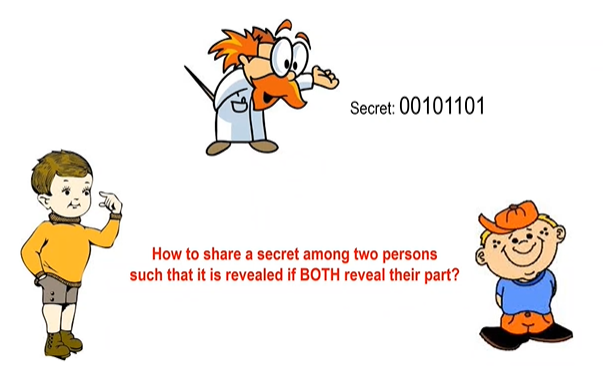
\includegraphics[scale=0.5]{2021-12-26-17-16-35.png}% chktex 8
\end{figure*}
Chi fornisce il segreto viene detto \textbf{dealer}, mentre chi riceve le porzioni del segreto sono detti \textbf{share}\@.\newline
Nel caso in cui avessimo diviso il segreto in parti uguali, è una pessima idea poiché per indovinare il segreto abbiamo \(\frac{1}{2^{N_{bit}}}\) probabilità di indovinare la password ed ora, avendo diviso il segreto in parti uguali, abbiamo una probabilità molto maggiore \(\frac{1}{2^{\frac{N_{bit}}{2}}}\) \@.
\subsection{XOR Secret Sharing}
Possiamo fare di meglio:\begin{enumerate}
	\item Prendi il segreto i.e.0010.1101;
	\item Genera una sequenza casuale \textbf{key} i.e.1011.0100;
	\item XOR il segreto e il valore casuale \textbf{one time pad} i.e.1001.1001;\newline
	      Fino ad ora abbiamo applicato un \emph{Vernam cipher}\@.
	\item Diamo ad uno share la sequenza casuale, mentre ad un altro diamo il valore dello XOR;\@
	\item L'unione fra gli share da la chiave\@.
\end{enumerate}
\begin{Importante}
	Il conoscere la chiave, cioè il valore casuale, non mi da alcuna informazione riguardante la chiave\@.\newline Lo stesso discorso vale per il valore dello XOR poiché, come dimostrato nel \textbf{perfect secrecy}, l'operatore di XOR tra una stringa pseudocasuale e un valore casuale non da informazioni su quale sia la password\@.\newline
	Questi due aspetti rappresentano un requisito di sicurezza\@.
\end{Importante}
\newpage
\subsection{Modular Secret Sharing}
Un altro possibile schema è quello di utilizzare le somme modulari:\begin{enumerate}
	\item Prendi il segreto S in bit, trasformalo in digit i.e.0010.1101\(rightarrow\)45;
	\item Genera \(RAND\mod{N}\) i.e.\(RAND\mod{256} \rightarrow  180\);
	\item Esegui \(S-RAND\mod{N}\) i.e. \(S-RAND\mod{256}\rightarrow  121\);
\end{enumerate}
\begin{Importante}
	Questo schema è equivalente ad One Time Pad poiché abbiamo sommato un numero pseudocasuale con un numero casuale (in modulo)\@. In altre parole, la probabilità di indovinare S conoscendo il valore casuale o il valore della somma è uguale alla probabilità di indovinare senza sapere nulla\@.
\end{Importante}
Questo metodo è più facile da implementare per essere condiviso con N shareholders\@. In particolare, genero 3 quantità truly random ed effettua la differenza tra il segreto e queste 3 quantità modulo N\@.
Nel caso un attacker, riuscisse ad ottenere un numero sufficiente di share non può comunque ottenere la password, ma al più la differenza tra il segreto e le shares non prese\@.\newline Da qui è possibile definire il concetto di \textbf{perfect secrecy}: un avversario, conoscendo n-1 shares deve ancora possedere la probabilità di indovinare il segreto pari a quella di indovinare il segreto da zero\@.
\section{Shamir Secret Sharing}
Fino ad ora abbiamo costruito uno schema detto (n,n) secret sharing scheme in cui il primo parametro è il numero delle persone necessarie a rilevare il segreto e il secondo parametro è il numero di parti:\@il segreto viene rilevato solo se tutte le n parti forniscono il segreto\@.\newline
Un altro schema è \textbf(t,n) secret sharing scheme:\@il segreto è rilevato quando qualsiasi t delle n parti fornisce il segreto\@. Questo secondo problema è molto più complicato del trivial secret sharing\@.
\subsection{Idea:\@Schema (2,n)}
Il problema è quello di modellare uno schema per cui, conoscendo 2 degli n shareholders, posso ricostruire il segreto\@. Questo problema è riconducibile a quello di conoscere quanti punti sono necessari per definire una linea:\@ovviamente 2\@.
\begin{figure*}[h]
	\centering
	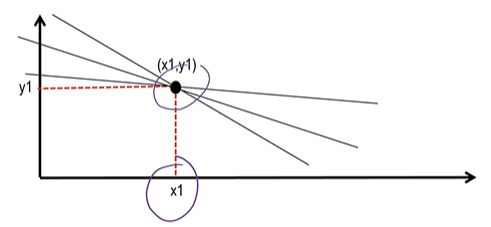
\includegraphics[scale=0.5]{2021-12-26-18-33-00.png}% chktex 8
\end{figure*}
Infatti conoscendo un solo punto (shares) ho infinite rette passanti per quel punto e quindi è impossibile ricondurci al segreto;\@tuttavia, conoscendo 2 punti (shares), tra essi passa solamente una sola retta e conseguentemente posso conoscere il segreto\@. Abbiamo comunque mantenuto la proprietà di poter avere un numero maggiore di 2 per ottenere il segreto, ma al minimo sono 2\@.
\subsection{Procedura: Schema\((2,n)\)}
\begin{itemize}
	\item \textbf{Dealer:} costruisce la linea:
	      \begin{enumerate}
		      \item Coefficiente a:\@scelto casualmente;
		      \item Segreto S:\@noto;
		            \begin{equation*}
			            \centering
			            y=S+ax
		            \end{equation*}
	      \end{enumerate}
	      Per esempio: \(a=15\quad S=39\)
	\item Distribuisci le shares ai n partecipanti scegliendo casualmente il valore \(x_{i}\) da introdurre nell'equazione della retta:
	      \begin{itemize}
		      \item Shareholder 1: \(x_{1}=1\rightarrow share=(1,54)\);
		      \item Shareholder 2: \(x_{2}=2\rightarrow share=(2,69)\);
		      \item Shareholder 3: \(x_{3}=3\rightarrow share=(3,84)\);
		      \item \dots
	      \end{itemize}
\end{itemize}
\begin{Importante}
	La y viene calcolata in base alla funzione della retta;\@tuttavia, i punti degli shareholder sono mantenuti con (x,y) e il valore delle \(x_{i}\) possono essere noti a priori a patto che la y sia nascosta\@.
\end{Importante}
\subsection{Procedura: Ricostruzione (2,n)}
\begin{itemize}
	\item Ricezione di due shares:\(P_{i}=(x_{i},y_{i})\quad P_{j}=(x_{j},y_{j})\);
	\item Interpola i punti per ricostruire l'equazione della retta:
	      \begin{equation*}
		      \centering
		      \frac{y-y_{i}}{y_{i}-y_{j}}=\frac{x-x_{i}}{x_{i}-x_{j}}
	      \end{equation*}
	      Ottenendo:
	      \begin{equation*}
		      \centering
		      y=y_{i}+\frac{x-x_{i}}{x_{i}-x_{j}}(y_{i}-y_{j})
	      \end{equation*}
	\item Bisogna sostituire \(x=0\) per ottenere il segreto \(y=S\);
\end{itemize}
\subsection{Estensione al caso \((t,n)\)}
Estendendo il discorso precedentemente introdotto, ci si riconduce al caso di polinomi di grado \(t-1\) unicamente definiti da \(t\) punti:
\begin{itemize}
	\item Linea:\@2 punti;
	\item Parabola (quadratic):\@3 punti;
	\item Cubiche:\@4 punti;
	\item \dots
\end{itemize}
\subsection{Generalizzazione: Schema \((t,n)\)}
\begin{itemize}
	\item \textbf{Dealer}:\
	      \begin{enumerate}
		      \item Genera un polinomio casuale \(p(x)\) di grado \(t-1\);
		      \item Imposta il segreto \(s\) come il termine noto del polinomio:
		            \begin{equation*}
			            p(x)=s+a_{1}x+a_{2}x^{2}+ \cdots +a_{t-2}x^{t-2}+a_{t-1}x^t-1
		            \end{equation*}
		            con s il segreto e i coefficienti delle x generati truly random;
		      \item Distribuisci uno share ad ogni shareholders:
		            \begin{equation*}
			            \centering
			            (x_{i},y_{i})\rightarrow y_{i}=p(x_{i})
		            \end{equation*}
	      \end{enumerate}
	\item \textbf{Ricostruzione}: Colleziona \(t\) shares su \(n\) disponibili e calcola il segreto utilizzando \emph{l'interpolazione di Lagrange} con \(x=0\):
	      \begin{equation*}
		      \centering
		      s=\sum_{shares\ x_i}{y_{i}\Lambda_{x_{i}}}\quad with\quad\Lambda_{x_{i}}=\Lambda_{x_{i}}(0)=\prod_{shares\ x_{k}\neq x_{j}}{\frac{-x_{k}}{x_{i}-x_{k}}}
	      \end{equation*}
	      L'interpolazione di Lagrange si basa sul concetto che qualsiasi polinomio di grande t-1 con t punti noti, può essere decomposto come:
	      \begin{equation*}
		      \centering
		      y=\sum_{i=1}^{t}{y_{i}\Lambda_{i}(x)}
	      \end{equation*}
	      In cui \(\Lambda_{i}(x)\) è la base del polinomio calcolata come:
	      \begin{equation*}
		      \centering
		      \Lambda_{i}(x)=\prod_{m=1,m\neq1}^{l}{\frac{x-x_{m}}{x_{i}-x_{m}}}\quad \Lambda_{i}(x_{i})=1;\quad \Lambda_{i}(x_{m})=0\quad for\ m\neq i
	      \end{equation*}
\end{itemize}
\subsection{Segretezza}
Per discutere di quanto sia sicuro questo schema dobbiamo ricordare che in questo ambito la segretezza è così definita:
\begin{center}
	\emph{Finché si conoscono (t-1) shares non si dovrebbe avere nessuna informazione sul segreto che stiamo condividendo.}
\end{center}
Lo schema di Shamir in questo senso non è sicuro poiché se conoscessi a priori il range in cui è compreso il segreto, potrei ciclare su uno share mancante per ottenere un segreto nel range voluto\@.
\begin{esempio}
	Effettuiamo uno schema (3,4) in cui per conoscere il segreto dobbiamo conoscere almeno 3 share su 4\@. Dato che utilizziamo l'interpolazione di Lagrange il polinomio sarà di grado \(t-1\) e il termine noto sarà \(s\):
	\begin{equation*}
		y=3 x^2+52 x+32;
	\end{equation*}
	Abbiamo 4 shareholders, quindi dobbiamo generare 4 punti,generando un valore casuale x e sostituendolo nell'equazione precedente. Avendo posto rispettivamente i valori \(1,2,3,4\), si ottengono i seguenti punti:
	\begin{equation*}
		(1,87),(2,148),(3,215),(4,288)
	\end{equation*}
	Ora, occorre calcolare i valori di lambda, supponendo di aver collezionato \(x_{1},x_{2},x_{3}\), come
	\begin{equation*}
		\centering
		\Lambda_{i}(x)=\prod_{m=1,m\neq1}^{l}{\frac{x-x_{m}}{x_{i}-x_{m}}}\quad \Lambda_{i}(x_{i})=1;\quad \Lambda_{i}(x_{m})=0\quad for\ m\neq i
	\end{equation*}
	Ottenendo:
	\begin{equation*}
		\Lambda_{1}(x)=\frac{(x-\text{x2}) (x-\text{x3}) }{(\text{x1}-\text{x2}) (\text{x1}-\text{x3}) }
	\end{equation*}
	\begin{equation*}
		\Lambda_{2}(x)=\frac{(x-\text{x1}) (x-\text{x3}) }{(\text{x2}-\text{x1}) (\text{x2}-\text{x3}) }
	\end{equation*}
	\begin{equation*}
		\Lambda_{3}(x)= \frac{(x-\text{x1}) (x-\text{x2}) }{(\text{x3}-\text{x1}) (\text{x3}-\text{x2}) }
	\end{equation*}
	Ora, per ricostruire il segreto occorre applicare
	\begin{equation*}
		\centering
		y=\sum_{i=1}^{t}{y_{i}\Lambda_{i}(x)}
	\end{equation*}
	Quindi:
	\begin{equation*}
		s=y_{1}\Lambda_{x_{1}}(0)+y_{2}\Lambda_{x_{2}}(0)+y_{3}\Lambda_{x_{3}}(0)=87(30)+148(-3)+215(1)=32
	\end{equation*}
	Ora supponiamo di non sapere uno share \emph(\(d\)) e vogliamo verificare se questo schema garantisce secrecy o meno\@. Sostituendo imponiamo:
	\begin{equation*}
		s=y_{1}\Lambda_{x_{1}}(0)+d\Lambda_{x_{2}}(0)+y_{3}\Lambda_{x_{3}}(0)= 476-3d
	\end{equation*}
	Ipotizziamo che il range in cui vive s è noto e compreso tra 0 e 100\@. Possiamo indovinare il segreto? Si, basta ciclare sulle d:\begin{itemize}
		\item Con \(d=125\rightarrow s=101\);
		\item Con \(d=126\rightarrow s=98\);
		\item Con \(d=127\rightarrow s=95\);
		\item Da varie prove si capisce che d è nel range \(126\leq d\leq 158\);
	\end{itemize}
	Quindi, conoscere 2 su 3 in uno schema 3 su 4 ci permette di escludere tutti i valori d non ammissibili\@.
\end{esempio}
\subsection{Real Shamir Secret Sharing}
Lo schema reale utilizza l'aritmetica modulare (con \(p\) numero primo) invece di quella reale e  le operazioni effettuate sia con il segreto sia con il polinomio devono essere scelti nel campo dei numeri primi\@.\newline
L'interpolazione rimane uguale\@.
\begin{Importante}
	La regola per scegliere il numero primo p deve essere più grande del dominio del segreto per avere un segreto uniformemente distribuito e non è necessario che sia grande\@.
\end{Importante}
\begin{esempio}
	La nuova costruzione corretta che utilizza il modulo è la seguente\@.\newline
	Supponiamo di avere un segreto \(s\in[0,100]\) in uno schema \((3,4) \) \@.
	\begin{enumerate}
		\item Scegliamo il primo numero primo maggiore dell'intervallo in cui è compreso s\@.
		      \begin{equation*}
			      p=101
		      \end{equation*}
		\item Il segreto che vogliamo inviare è:\@ \(s=32\).
		\item Il polinomio sarà di grado \(t-1\) e con termine noto \(s\):\begin{equation*}
			      y=Mod[32+52x+3x^{2},101]=(32+52x+3x^{2})\mod{101}
		      \end{equation*}
		\item Generiamo i valori per gli shareholders:
		      \begin{equation*}
			      \begin{matrix}
				      x_{1}=1\rightarrow y_{1}=y/.{x\rightarrow x_{1}}=87 \\
				      x_{2}=2\rightarrow y_{2}=y/.{x\rightarrow x_{2}}=47 \\
				      x_{3}=3\rightarrow y_{3}=y/.{x\rightarrow x_{3}}=13 \\
				      x_{4}=6\rightarrow y_{4}=y/.{x\rightarrow x_{4}}=48 \\
			      \end{matrix}
		      \end{equation*}
		\item Calcoliamo i valori \(\Lambda_{i}(0) \) presupponendo di conoscere le share di \(1,2,4\), sostituendo \(x=0\) e ovviamente considerando il modulo:
		      \begin{equation*}
			      \begin{matrix}
				      \Lambda_{1}(x)= Mod[(0-x{2})*(0-x_{4})*PowerMod[(x_{1}-x{2})*(x_{1}-x{4}),-1,101],101]=63 \\
				      \Lambda_{2}(x)= Mod[(0-x{1})*(0-x_{4})*PowerMod[(x_{2}-x{1})*(x_{2}-x{4}),-1,101],101]=49 \\
				      \Lambda_{4}(x)= Mod[(0-x{1})*(0-x_{2})*PowerMod[(x_{4}-x{1})*(x_{4}-x{2}),-1,101],101]=91
			      \end{matrix}
		      \end{equation*}
		      \begin{Importante}
			      \begin{equation*}
				      \centering
				      \Lambda_{i}(x)=\prod_{m=1,m\neq1}^{l}{\frac{x-x_{m}}{x_{i}-x_{m}}}\quad \Lambda_{i}(x_{i})=1;\quad \Lambda_{i}(x_{m})=0\quad for\ m\neq i
			      \end{equation*}
			      Questa formula imporrebbe di scrivere il denominatore sotto il segno di frazione, ma questo non è possibile se si effettua il modulo\@. Quindi, quello che occorre fare è effettuare l'inversa del modulo: in mathematica si utilizza PowerMod. Per esempio per \(\Lambda_{1}(0)\):
			      \begin{equation*}
				      \Lambda_{1}(x)= Mod[(0-x{2})*(0-x_{4})*PowerMod[(x_{1}-x{2})*(x_{1}-x{4}),-1,101],101]=(\frac{(0-x{2})*(0-x_{4})}{(x_{1}-x{2})*(x_{1}-x{4})})\mod{p}
			      \end{equation*}
			      In cui:
			      \begin{equation*}
				      \frac{1}{(x_{1}-x_{2})*(x_{1}-x_{4})}\mod{101}=
				      {((x_{1}-x_{2})(x_{1}-x{4}))}^{-1}\mod{101}
			      \end{equation*}
		      \end{Importante}
		\item La forma per ricostruire il segreto è la seguente:
		      \begin{equation*}
			      Mod[y_{1}\Lambda_{1}(x)+y_{2}\Lambda_{2}(x)+y_{3}\Lambda_{3},101]=(y_{1}\Lambda_{1}(x)+y_{2}\Lambda_{2}(x)+y_{3}\Lambda_{3})\mod{101}=32
		      \end{equation*}
		\item Verifichiamo ora che sia unconditionally secure:\@finché ho anche uno share mancante, allora il segreto potrebbe essere qualsiasi\@. In particolare, supponiamo che non sia noto \(d=y_{1}\) e cicliamo su d da 0 a 100, sapendo che il segreto è compreso in questo intervallo:
		      \begin{equation*}
			      Mod[d*\Lambda_{1}(x)+y_{2}*\Lambda_{2}(x)+y_{3}*\Lambda_{3}(x)/.{d\rightarrow Range[0,100]}]
		      \end{equation*}
		      Come osserviamo i possibili valori sono molteplici e uniformemente distribuiti tra 0 e 100:
	\end{enumerate}
\end{esempio}
\begin{center}
	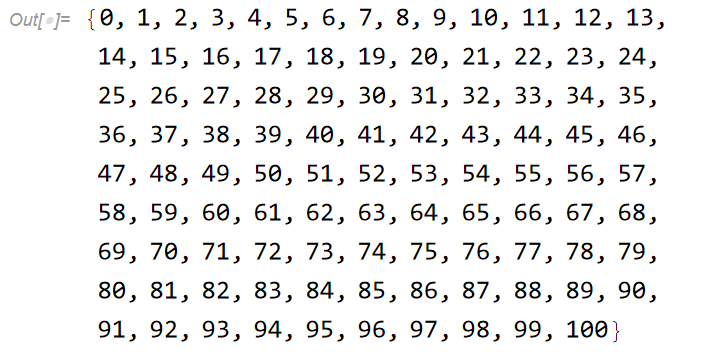
\includegraphics[width=0.48\textwidth]{2021-12-29-10-57-00.png}% chktex 8
\end{center}
\section{Secret Sharing: Details}\begin{itemize}
	\item Gli shares non possono essere più piccoli del segreto, ma al più larghi quanto il segreto\@. A tale scopo, intuitivamente la conoscenza di uno share deve aggiungere informazioni al segreto, riducendone l'entropia\@. Quindi, dati t-1 shares, non si può determinare nulla riguardo al segreto ed, inoltre, lo share finale deve contenere quanta più informazione quanta ne ha il segreto stesso\@.
	\item Shamir Scheme Ideal quando lo share ha la stessa dimensione del segreto\@. Vi sono esempio di schemi con chiavi maggiore del segreto come lo schema di \emph{Blackley}\@.
\end{itemize}
\section{Secret Sharing for secure multiparty computation}
\subsection{Homomorphic Property}
\setlength\intextsep{0pt}
\begin{wrapfigure}[12]{R}[0pt]{0pt}
	\centering
	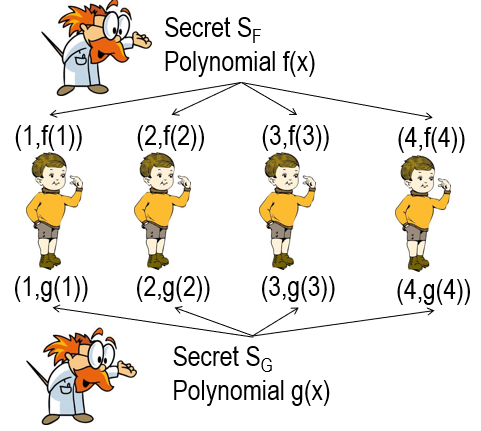
\includegraphics[scale=0.5]{2021-12-29-21-48-24.png}% chktex 8
\end{wrapfigure}
Assumiamo uno schema (3,4) scheme e supponiamo di avere un Dealer che genera un segreto \(S_{F}\) e un polinomio \(f(x)\).
Il dealer condividere a 4 shareholders (parties) gli shares.
In parallelo, un altro Dealer genera un altro segreto \(S_{G}\) con un altro polinomio \(g(x)\) e anche lui genera e condivide gli shares\@.\newline
Il nostro obiettivo è calcolare \(S_{F}+S_{G}\):\@ approccio sarebbe quello di ricostruire inizialmente entrambi i segreti per poi effettuarne la somma;\@tuttavia grazie allo schema di Shamir \textbf{la somma degli shares è uguale alla somma dei segreti} (ovviamente applicando la formula di ricostruzione) \@.
Quindi, la proprietà homomorphic risiede nel fatto che è possibile calcolare \(S_{F}+S_{G}\) senza sapere i due segreti: effettuare calcoli sui segreti senza rivelare niente dei segreti\@.
\subsection{SMC:\@Secure Multiparty Computation}
SMC (\textbf{Secure Multiparty Computation}) l'obiettivo è quello di calcolare il risultato di una funzione senza rivelare i dati in input\@. Funziona nel seguente modo:
\begin{itemize}
	\item Date \(N\) parti \(P_{1},P_{2},\dots,P_{n}\) ognuna delle quali con valore \(z_{i}\);
	\item Calcola la funzione \(f(z_{1},z_{2},\dots,z_{n})\) \@. Il suo risultato è pubblico, ma non si deve dare alcuna informazione riguardo agli input;
	\item \emph{se l'operazione è una funzione lineare al più pesata da dei coefficienti, allora diventa banale e identico al Secret Sharing Scheme classico};
\end{itemize}
Schematicamente, senza l'utilizzo di SMC:\@
\begin{figure}[h]
	\centering
	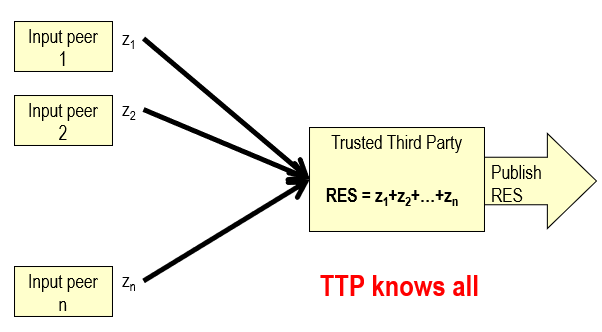
\includegraphics[scale=0.5]{2021-12-29-23-00-13.png}% chktex 8
\end{figure}
La terza parte deve essere trusted e conosce tutto il segreto\@.\newpage
Al contrario, con SMC si ha l'assenza di trusted third parties poiché il segreto è noto solo dall'unione dei privacy peers (\emph{applicando la proprietà homomorphic}):
\begin{figure}[h]
	\begin{center}
		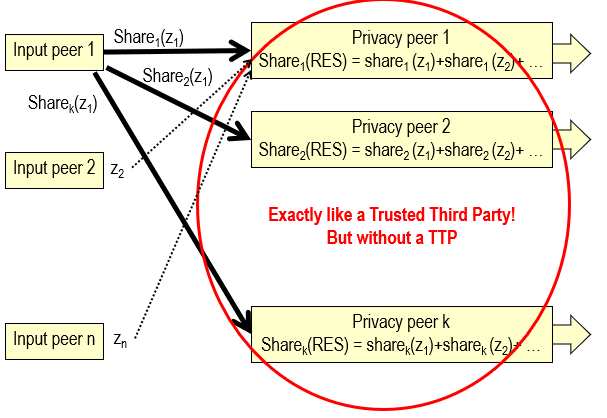
\includegraphics[scale=0.4]{2021-12-29-23-03-44.png}% chktex 8
	\end{center}
\end{figure}
\begin{Importante}
	\begin{itemize}
		\item Si necessitano almeno di 3 peers poiché se ce ne fossero 2 ad una parte basterebbe calcolare il segreto tramite complementarietà;
		\item Ci possono essere molteplici end users;
		\item Ci devono essere almeno 2 privacy peers, ma più ce ne sono maggiore è la sicurezza e robusto alle collisione;
		\item Soglia sul numero di peers pari a \(2\leq t\leq k\) se è uno schema (t,k).
	\end{itemize}
\end{Importante}
\subsection{Costruzione}
\begin{itemize}
	\item Input peer i:\begin{enumerate}
		      \item Input data \(z_{i}\);
		      \item Genera un polinomio \(p_{i}(x)\) di grado \(t-1\) con \(z_{i}\) termine noto;
		      \item Invia privatamente gli shares \(p_{i}(1),\dots,p_{i}(k)\) ai privacy peer \(1,\dots,k\);
	      \end{enumerate}
	\item Privacy peer \(m\):\begin{enumerate}
		      \item Collezione gli input shares \(p_{1}(m),\dots,p_{n}(m)\);
		      \item Calcola \(RES=p_{1}(m)+\dots,p_{n}(m)\);
		      \item Pubblica lo share aggregato \(RES(m)\);
	      \end{enumerate}
	\item Public:\begin{enumerate}
		      \item Ricostruisci RES da un numero sufficiente di \(RES(m)\) con l'interpolazione di Lagrange.
	      \end{enumerate}
\end{itemize}
\begin{esempio}
	Versione distribuita dello schema precedente:\newline
	\begin{tabular}{c c}
		(1)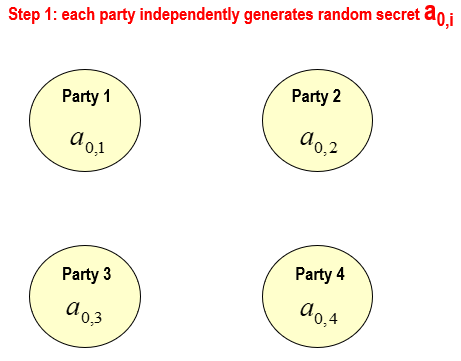
\includegraphics[scale=0.5]{2021-12-29-23-40-26.png}% chktex 8
		 &
		(2)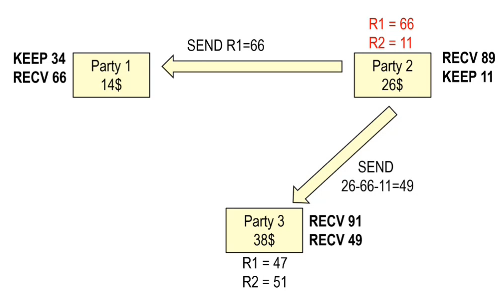
\includegraphics[scale=0.5]{2021-12-29-23-43-20.png}% chktex 8
		\\
		(3)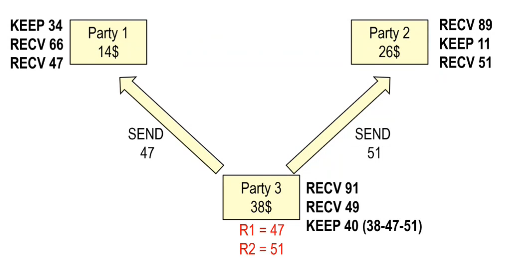
\includegraphics[scale=0.5]{2021-12-29-23-45-01.png}% chktex 8
		 &
		(4)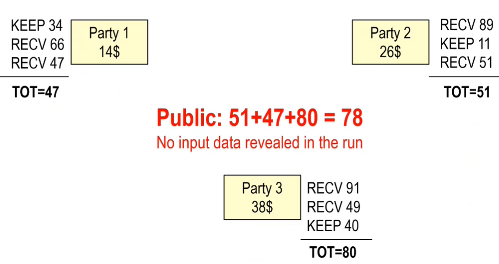
\includegraphics[scale=0.5]{2021-12-29-23-47-08.png}% chktex 8
		\\
	\end{tabular}
\end{esempio}
\chapter{Verifiable Secret Sharing}
Quando si immette uno share non è possibile capire se è un valore corretto o meno (\emph{cheating})\@. Il nostro obiettivo è capire se vi sono delle tecniche per verificare le operazioni crittografiche\@.\newline
L'\textbf{honest-but-curious model} è un modello in cui un attacker segue le regole per ottenere il segreto (quello classico è quello in cui l'attacker cheatta e questo viene detto malicious) \@. Quindi, il nostro obiettivo è quello di avere dei modi per rilevare e bloccare i cheaters che possono essere sia i dealer che i players\@.\newline
Si ha bisogno di verifiable secret sharing quando un party può verificare qualora il dealer share è consistente (\emph{rilevare malicious dealer}) oppure le parti possono verificare qualora il segreto rivelato è consistente (\emph{detect cheating parties}) \@.
\section{VSS:\@Feldman VSS Scheme}
\subsection{Feldman Scheme:\@dealer}
\begin{itemize}
	\item Inizia con un ordinary Shamir scheme:\begin{enumerate}
		      \item Genera un polinomio casuale \(p(x)\) con grado \((t-1)\), con \(P(0)=s\):
		            \begin{equation*}
			            p(x)=s+a_{1}x+a_{2}x^{2}+\cdots+a_{t-2}x^{t-2}+a_{t-1}x^{t-1}
		            \end{equation*}
		      \item Distribuisci uno share ad ognuna delle n parti:\begin{equation*}
			            (x_{i},y_{i})\quad y_{i}=p(x_{i})
		            \end{equation*}
	      \end{enumerate}
	\item Per ogni coefficiente del polinomio pubblichiamo in chiaro i seguenti termini detti \textbf{commitments}:\begin{equation*}
		      c_{0}=g^{s};c_{1}=g^{a_{1}};\ldots;c_{t-1}=g^{a_{t-1}}\mod{p}
	      \end{equation*}
	      \begin{Importante}
		      Se utilizziamo \(p\), grande numero primo, e i coefficienti del polinomio in \emph{Large Fields} allora i coefficienti \(c_{i}\) non rivelano nulla del segreto poiché si basano sul problema del discrete log (sono difficili da calcolare).
	      \end{Importante}
\end{itemize}
\subsubsection{Commitments}
Un commitment è una costruzione crittografica che deve possedere due proprietà:\begin{itemize}
	\item \emph{Hiding}: un receiver, ottenuto il commitment, non dovrebbe conoscere nulla riguardo il segreto; \textbf{COMMIT PHASE}
	\item \emph{Binding}: il commitment può essere aperto solo con il valore del segreto\@. Quindi, il mittente non può barare e cambiarlo. \textbf{REVEAL PHASE}
\end{itemize}
Anche \(C=H(x)\) è una sorta di commitment poiché possiede entrambe le proprietà, ma in aggiunta fornisce computationally hiding e computationally binding (\emph{con abbastanza tempo posso trovare una collisione})\@.\newline
Il Feldman Commitment \(c=g^{x}\) è un commitment:\begin{itemize}
	\item Hiding computazionale:\begin{enumerate}
		      \item Dato \(c=g^{x}\mod{p}\), computazionalmente legato al ricevitore senza conoscere \(x\) (\emph{x deve essere preso in intervallo grande});
	      \end{enumerate}
	\item Perfectly Binding:\begin{enumerate}
		      \item Il mittente non può trovare alcun \(x'\) tale che \(g^{x'}=c\);
		      \item
	      \end{enumerate}

\end{itemize}
\begin{Importante}
	Feldman VSS è solo computazionalmente sicuro\@. Ciò implica che se s è piccolo, \(c_{0}=g^{s}\) rivela informazioni sul segreto.
\end{Importante}
\subsection{Feldman Scheme:verifier}
\begin{itemize}
	\item La parte \(i\) riceve lo share \((x_{i},y_{i})\):\begin{enumerate}
		      \item Le altre parti possono verificare se la parte \(i\) è onesta senza sapere il segreto \(s\);
		      \item Le altre parti, dato che il dealer in questo caso è onesto, possono calcolare:\begin{align*}
			            c_{0}\cdot c_{1}^{x_i}\cdot c_{2}^{x_{i}^{2}}\cdot c_{t-1}^{x_{i}^{t-1}} & =                                                                                                           \\                                                       & =(g^{s})\cdot {(g^{a_{1}})}^{x_{i}}\cdot {(g^{a_{2}})}^{x_{i}^2}\cdot\cdots\cdot {(g^{a_{t-1}})}^{x_{i}^{t-1}}= \\
			                                                                                     & = g^{s}\cdot g^{a_{1}\cdot x_{i}}\cdot g^{a_{2}\cdot x_{i}^2}\cdot\cdots\cdot g^{a_{t-1}\cdot x_{i}^{t-1}}= \\
			                                                                                     & = g^{s+a_{1}x{i}+a_{2}x_{i}^2+\cdots +a_{t-1}x_{i}^{t-1}}=g^p(x_{i})
		            \end{align*}
		      \item così facendo le altre parti effettuano una homomorphic computation di \(p(x_{i})\) all'esponente ottenendo \(g^{p(x_{i})}\);
		      \item Ora per verificare le parti hanno \(y_{x_{i}}\), calcolando \(g^{y_{x_{i}}}\) e se è uguale a quello calcolato al passo precedente, allora lo share è verificato\@.
	      \end{enumerate}
\end{itemize}
\section{Pedersen Commitment}
Non è possibile avere uno schema perfectly hiding:\@uno schema in cui un commitment sia contemporaneamente perfectly hiding e perfectly binding\@.\newline Tuttavia, esistono commitment che sono perfectly hiding, ma computationally binding\@. L'approccio di Feldman funzionava poiché si ha un commitment che è anche homomorphic\@.\newline
Quindi, vogliamo uno scheme perfectly hiding, ma che sia anche homomorphic: \textbf{Pedersen Commitment}\@.
\begin{Definizione}[Pedersen Commitment] Dati \(g\) e \(h\) pubblici\@:
	\begin{equation*}
		\centering
		Commit(a,r)=g^{a}\cdot h^{r}\mod{p}
	\end{equation*}
	In cui \(a\) è il segreto, \(r\) numero scelto truly random.
\end{Definizione}
Abbiamo ottenuto la proprietà homomorphic poiché:
\begin{align*}
	Commit(a+b,r_{a}+r_{b}) & =                                      \\
	                        & =g^{a}h^{r_{a}}\cdot g^{b}h^{r_{b}}=   \\
	                        & = Commit(a,r_{a})\cdot Commit(b,r_{b})
\end{align*}
Abbiamo ottenuto anche il perfectly hiding\@. Infatti, dato il commitment \(c=g^{a}h^{r}\) questo permette di nascondere qualsiasi valore di \(a\):\@ per qualsiasi \(a'\neq a\), possiamo trovare un unico \(r'\) tale che:\begin{equation*}
	Commit(a',r')=g^{a'}h^{r'}=g^{a}h^{r}=Commit(a,r)
\end{equation*}
Questo commitment è solamente computationally binding:\@il mittente non dovrebbe essere in grado di trovare un \(a'\), ma si può arrivare ad un trapdoor commitment scheme\@.
\begin{itemize}
	\item Sia \(h=g^{w}\) i.e.\(w=\log_{g}{h}\);
	\item Sappiamo \(a,r\), ci viene dato \(a'\) e cerchiamo un \(r'\) tale che:
	      \begin{align*}
		      g^{a}h^{r}=g^{a'}h^{r'} & \Longrightarrow g^{a}g^{wr}=g^{a'}g^{wr'}\Longrightarrow \\
		                              & \Longrightarrow g^{a+wr}=g^{a'+wr'}\Longrightarrow       \\
		                              & \Longrightarrow a+wr=a'+wr' \mod{q}\Longrightarrow       \\
		                              & \Longrightarrow r'=w^{-1}(a-a'+wr)=r'=(a-a')w^{-1}+r
	      \end{align*}
\end{itemize}
\section{Pedersen VSS:dealer}
\begin{itemize}
	\item Genera due polinomi casuali:\begin{align*}
		      f(x)  & =s+a_{1}x+a_{2}x^2+\cdots +a_{t-1}x^{t-1} \\
		      f'(x) & =r+b_{1}x+b_{2}x^2+\cdots +b_{t-1}x^{t-1}
	      \end{align*}
	\item Dai ad ogni parte lo share \(x_{i},y_{i},z_{i}\)
	      \begin{align*}
		      y_{i} & =f(x_{i})=s+a_{1}x_{i}+\cdots +a_{t-1}x^{t-1}  \\
		      z_{i} & =f'(x_{i})=r+b_{1}x_{i}+\cdots +b_{t-1}x^{t-1}
	      \end{align*}
	\item Pubblica i commitment di Pedersen:\begin{align*}
		      c_{0}   & =g^{s}h^r               \\
		      c_{1}   & =g^{a_{1}}h^{b_{1}}     \\
		      \vdots                            \\
		      c_{t-1} & =g^{a_{t-1}}h^{b_{t-1}}
	      \end{align*}
\end{itemize}
\section{Pedersen VSS:\@verifier}
\begin{itemize}
	\item La parte i-esima riceve lo share \(x_{i},y_{i},z_{i}\);
	\item Verifica in \(\mod{p}\) che:\begin{align*}
		      c_{0}\cdot c_{1}\cdot x_{i}\cdot \cdots \cdot c_{t-1}^{x_{i}^{t-1}} & ={(g^{s}h^{r})}\cdot {(g^{a_{1}}h^{b_{1}})}^{x_{i}}\cdot\cdots\cdot {(g^{a_{t-1}}h^{b_{t-1}})}^{x_{i}^{t-1}}=                                                  \\
		                                                                          & =g^{s}\cdot g^{a_{1}x_{i}}\cdot g^{a_{2}x_{i}^2}\cdot\cdots\cdot g^{a_{t-1}x_{i}^{t-1}}\cdot h^{r}\cdot h^{b_{1}x_{i}}\cdot\cdots\cdot h^{b_{t-1}x_{i}^{t-1}}= \\
		                                                                          & =g^{s+a_{1}x_{i}+a_{2}x_{i}^2+\cdots+ a_{t-1}x_{i}^{t-1}}\cdot h^{r+b_{1}x_{i}+b_{2}x_{i}^2+\cdots+b_{t-1}x_{i^{t-1}}}=                                        \\
		                                                                          & =g^{y_{i}}h^{z_{i}}
	      \end{align*}
	\item Se l'equazione è soddisfatta allora siamo riusciti a verificare;
\end{itemize}
\newpage
\section{Distributed Key Generation}
Nei sistemi crittografici basati su DLog, si ha: \(x\) chiave privata e \(g^{x}\) chiave pubblica\@. Vogliamo generare una coppia \((Pub_{K},Priv_{K})\) tale che tutti conoscono \(Pubb_{K}\), ma nessuno conosce \(Priv_{K}\).\\ Ciò ci è utile in tutti i casi in cui non vogliamo rilevare la chiave privata o deve essere ricostruita in seguito\@.\newline
Lo schema che realizza questa idea è chiamato \textbf{DKG} \emph{Distributed Key Generation}\@.\newline
\begin{tabularx}{0.99\textwidth}{X X}
	(1)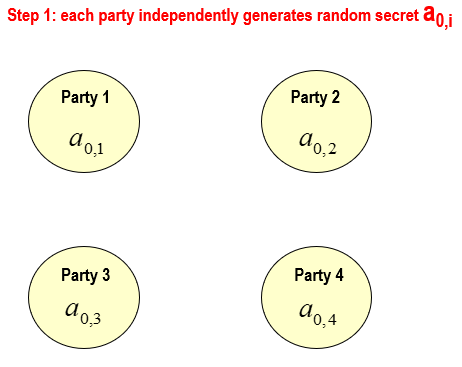
\includegraphics[scale=0.4]{2022-01-02-15-56-05.png}% chktex 8
	 &
	(2)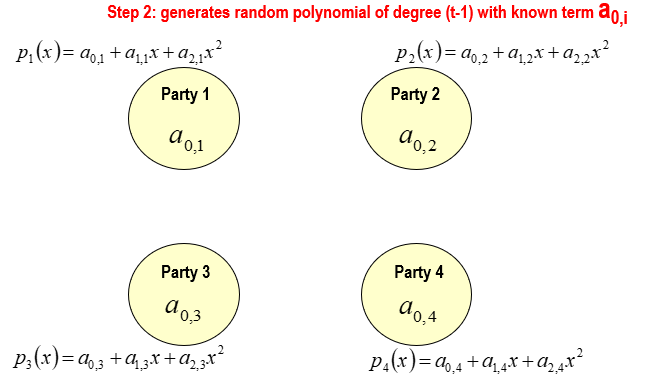
\includegraphics[scale=0.4]{2022-01-02-15-59-26.png}% chktex 8
	\\
	(3)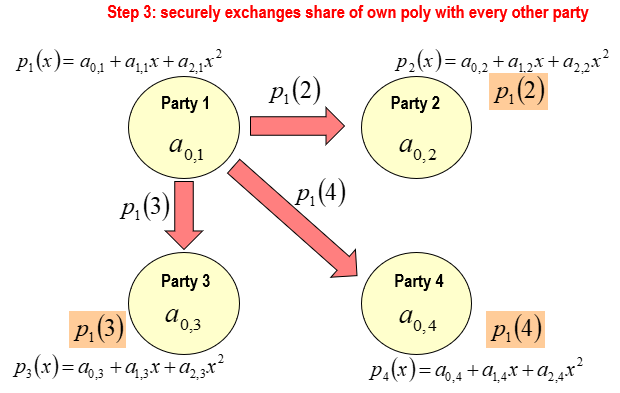
\includegraphics[scale=0.4]{2022-01-02-15-59-59.png}% chktex 8
	 &
	(4)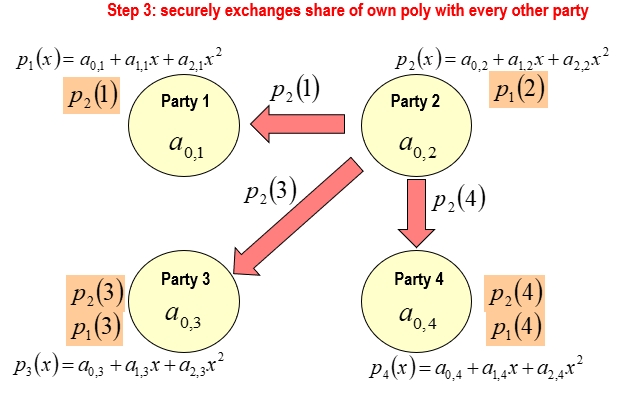
\includegraphics[scale=0.4]{2022-01-02-16-00-20.png}% chktex 8
	\\
	(5)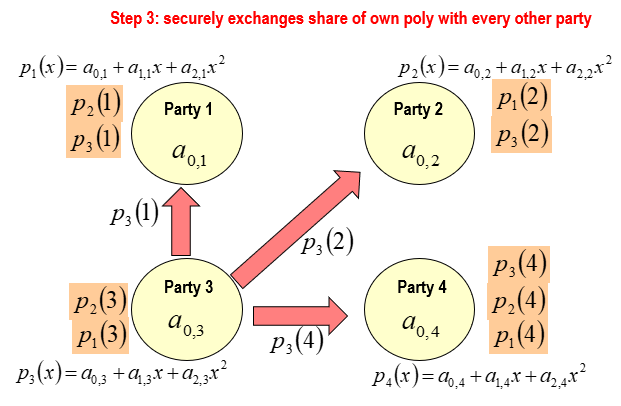
\includegraphics[scale=0.4]{2022-01-02-16-04-23.png}% chktex 8
	 &
	(6)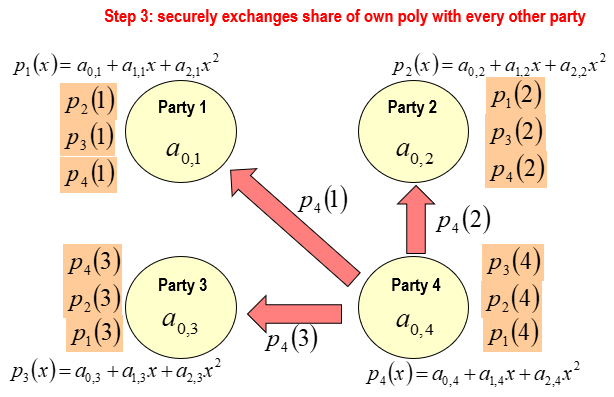
\includegraphics[scale=0.4]{2022-01-02-16-01-46.png}% chktex 8
	\\
	(7)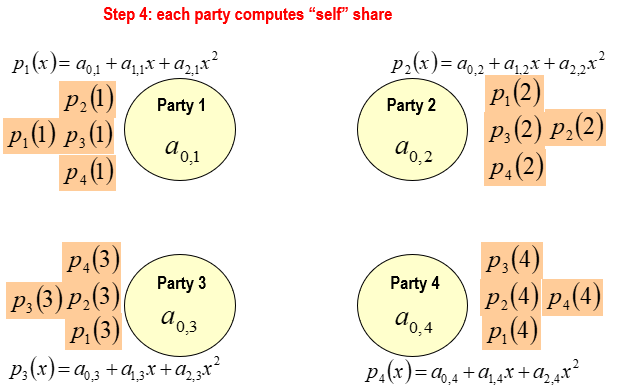
\includegraphics[scale=0.4]{2022-01-02-16-05-51.png}% chktex 8
	 &
	(8)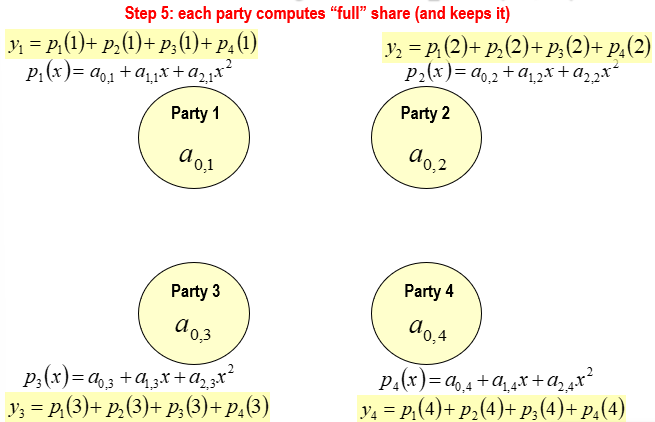
\includegraphics[scale=0.4]{2022-01-02-16-06-25.png}% chktex 8
	\\
	(9)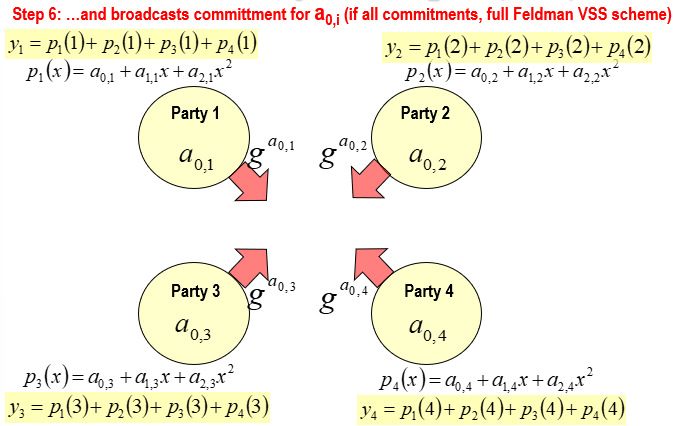
\includegraphics[scale=0.4]{2022-01-02-16-07-44.png}% chktex 8
	 &
	(10)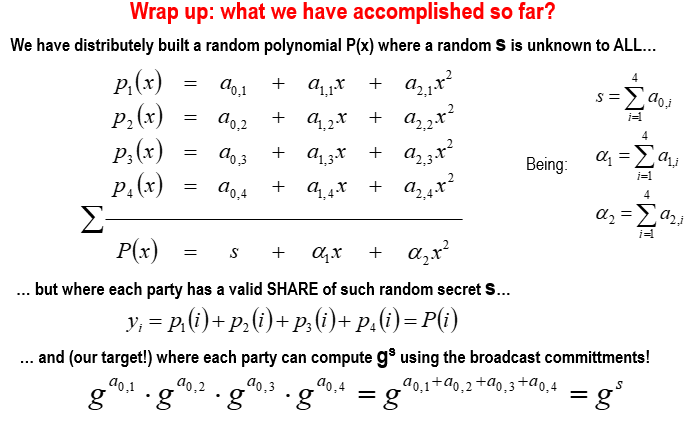
\includegraphics[scale=0.4]{2022-01-02-16-27-48.png}% chktex 8
\end{tabularx}
\chapter{Multiplicative Group\(\mod{p}\)}
\section{Gruppo}
Un \textbf{gruppo} \((G,\circ )\) è una struttura algebrica in cui \(G\) definisce l'insieme degli elementi (\emph{membri del gruppo}) e \(\circ \) è l'operazione del gruppo\@. Questa operazione deve soddisfare:\begin{itemize}
	\item \textbf{Chiusura}:\@presi due elementi \(g_{1},g_{2}\) del gruppo, allora \(g_{x}=g_{1}\circ g_{2}\) deve appartenere al gruppo;
	\item \textbf{Identità}:\@deve esiste un membro del gruppo tale che \(g\circ I = I\circ g=g\);
	\item \textbf{Inversa}:\@per ogni \(g\) esiste \(g^{-1}\) tale che \(g\circ g^{-1}=I\);
	\item \textbf{Associativa}:\@per qualsiasi \(g_{1},g_{2},g_{3}\) deve valere \((g_{1}\circ g_{2})\circ g_{3}=g_{1}\circ (\circ g_{3})\)
\end{itemize}
Inoltre, se l'operazione è anche commutativa, si ha un \textbf{Gruppo Abeliano}\@.
\subsection{Gruppo \(Z_{p}^{*}\)}
\(Z_{p}^{*}\) è la sintassi utilizzata per indicare il gruppo moltiplicativo modulo p:\@gli elementi di questo gruppo \textbf{finito} sono \(p-1\) composti da \( \{ 1,2,\ldots,p-1\} \) e l'unica operazione è la moltiplicazione (\emph{se l'avessimo considerata avremmo avuto un campo \(F_{p}\)})\@.\newline
Infatti, questo insieme di elementi con questa operazione, è un gruppo poiché è chiuso, è associativo, identità e commutatività (Gruppo Abeliano) e presenta l'inversa\@.
\begin{esempio}[\(Z_{11}^{*}\)]
	\begin{itemize}
		\item \(p-1=10\) elementi:\( \{1,2,3,4,5,6,7,8,9,10 \} \);
		\item Inverse in modulo p:\begin{align*}
			       & \Rightarrow 1\rightarrow 1                        \\
			       & \Rightarrow 2\rightarrow 6\quad & 6 \rightarrow 2 \\
			       & \Rightarrow 3\rightarrow 4\quad & 4 \rightarrow 3 \\
			       & \Rightarrow 5\rightarrow 9\quad & 9 \rightarrow 5 \\
			       & \Rightarrow 7\rightarrow 8\quad & 2 \rightarrow 7 \\
			       & \Rightarrow 10\rightarrow 10
		      \end{align*}
		\item Per grandi gruppi si utilizza l'algoritmo di Euclide esteso.
	\end{itemize}
\end{esempio}
\subsection{Gruppi moltiplicativi:exponentiation}
L'esponenziazione è una operazione che appartiene al gruppo \(Z_{p}^{*}\) poiché è l'applicazione della stessa operazione moltiplicativa più volte:\(x^{k}=x\circ x\circ x\circ x\circ \ldots \circ x\)(k volte).
\begin{Definizione}[Generatore di un Gruppo]
	Il generatore del gruppo è un valore \(g\) tale che \( \{g^{0},g^{1},\ldots ,g^{m-1} \} \) siano tutti gli elementi del gruppo
\end{Definizione}
\begin{Importante}
	Se \(m\) è primo, allora qualsiasi membro del gruppo è un generatore ad eccezione dell'identità\@.\\
	\(Z_{p}^{*}\) non è un \textbf{Prime-Order Group} infatti se \(p\) è primo, non lo è \(p-1\).
\end{Importante}
\newpage
\begin{esempio}[\(Z_{11}^{*}\)]
	\begin{itemize}
		\item \(p-1=10\) elementi:\( \{1,2,3,4,5,6,7,8,9,10 \} \);
		\item Quali sono i generatori? \( \{g^{1},g^{2},g^{3},\ldots ,g^{10}\} \)?
		\item \begin{align*}
			      g=2\rightarrow \{2,4,8,5,10,9,7,3,6,1\}\quad & \text{OK,è un generatore}                                \\
			      g=3\rightarrow \{3,9,5,4,1,3,,9,5,4,1\}\quad & \text{\textcolor{red}{NO, è un sottogruppo di ordine 5}} \\
			      etc\ldots
		      \end{align*}
		\item La cardinalità di sottogruppi deve essere uno dei fattori del numero degli elementi del gruppo: se \((p-1)=kq\) è il numero di elementi, allora potremmo incontrare sottogruppi di cardinalità \(k\) o \(q\).
	\end{itemize}
\end{esempio}
\section{Strong Primes}
In crittografia siamo interessati a prendere \emph{strong primes}.
\begin{Definizione}
	Un numero primo \(p\) è detto \textbf{strong prime} se \(p=2q+1\) con \(q\) numero primo.
\end{Definizione}
Quindi, qualsiasi sia \(x\) ad eccezione di 1 e p-1:\begin{itemize}
	\item Genera l'intero gruppo;
	\item Genera un sottogruppo di ordina primo q.
\end{itemize}
\section{Quadratic Residue Subgroup}
\begin{Definizione}
	Sia \(x\in Z_{p}^{*}\) è un \textbf{quadratic residue} se ammette la radice quadrata in \(Z_{p}^{*}\).
\end{Definizione}
Per esempio esiste \(a\) tale che \(a^{2}\mod{p}=x\).\newline
Se soddisfo la definizione allora sono il generatore di un sottogruppo;\@altrimenti sono il generatore dell'intero gruppo.
\begin{itemize}
	\item QR forma un sottogruppo di ordine \(\frac{p-1}{2}\);
	\item QR Test: \textbf{Legendre Symbol}:\(a\in QR\) se \(a^{\frac{p-1}{2}}\mod{p}=1\) (se pari a \(-1\) allora sono un generatore)
\end{itemize}
\begin{Importante}
	Vedere applicazioni nel file matematica 41-vss-example-1-qr e -correct.
\end{Importante}
\chapter{Threshold and policy-based cryptography}
La \textbf{threshold cryptography}è un tipo di crittografia in cui l'encryption o una signature può essere decryptata solo quando vi sono un certo numero di partecipanti. Si può anche definire come group crypto composta da VSS con tecniche standard di criptografia\@.
\section{Threshold Encryption}
\subsection{Public Key Encryption with DLOG}
Vogliamo applicare il DLOG con la public encryption: schema El Gamal (DH adattato)\@. Si è fatta questa scelta poiché viene facilmente implementato nelle curve ellittiche\@.
\subsection{El-Gamal:background}
Lo schema di El-Gamal modifica il protocollo di accordo delle chiavi in un cipher asimmetrico\@.
\subsection{El-Gamal:Sketch}
\begin{itemize}
	\item Operazioni in \(\mod{p}\) con \(p\) numero primo elevato;
	\item \(g\) generatore di gruppo;
	\item \(s\) chiave privata;
	\item \(h=g^{s}\) chiave pubblica;
	\item \(r\) valore casuale;
\end{itemize}
\begin{Importante}
	\begin{itemize}
		\item \(g^{s},g^{r}\) noti a tutti:\@il primo pubblico, il secondo nel ciphertext;
		\item \(s\) noto solo dal receiver;
		\item \(r\) noto solo dal transmitter;
		\item \(g^{sr}\) nessun altro può calcolarlo
	\end{itemize}
\end{Importante}
Quindi per \textbf{cifrare}:\begin{equation*}
	(R,c)=(g^{r},m\cdot h^{r})
\end{equation*}
Per \textbf{decifrare}:\begin{equation*}
	m=c\cdot R^{-s}=\frac{c}{{(g^{r})}^{s}}=\frac{m\cdot h^{r}}{g^{rs}}=\frac{m\cdot g^{sr}}{g^{rs}}
\end{equation*}
\newpage
\subsection{Asymmetric Cryptography}
Schema su come si applica El-Gamal:
\begin{figure*}[h]
	\centering
	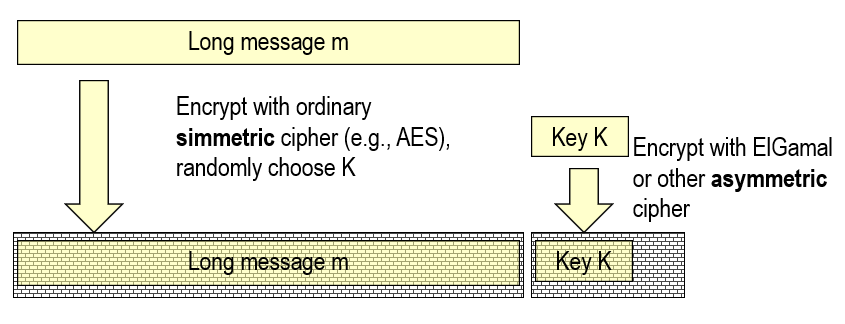
\includegraphics[scale=0.5]{2022-01-03-15-37-08.png}% chktex 8
\end{figure*}
\subsection{ECIES=Hybrid Encryption 5g}
\textbf{ECIES} sta per \emph{Elliptic Curve Integrated Encryption Scheme} e venne per la prima volta standardizzato nell'IMSI del 5G\@. Assumiamo che nella nostra SIM ho installato la chiave pubblica del provider della SIM (Trusted) \(g^{HN}\) (Home Network)\@. Nel momento dell'autenticazione \textbf{Encrypt-then-MAC}:\begin{itemize}
	\item generiamo \(x\) casuale, il coefficiente ephemeral \(g^{x}\);
	\item calcoliamo \(K=HKDF(g^{HNx})\) ed inviamo \(AES_{k}(SUP)\) (SUP è l'IMSI);
	\item aggiungiamo \(HMAC\) (integrità);
	\item Il messaggio sarà quindi \(({g}^{x},HMAC(AES_{k}(MSG)))\)
\end{itemize}
In ricezione:\begin{itemize}
	\item Riceviamo \(({g}^{x},HMAC(AES_{k}(MSG)))\):\begin{enumerate}
		      \item Con \({g}^{x}\) e la chiave privata dell'Home Network ricostruiamo la chiave \({(g^{x})}^{HN}\);
		      \item Deriviamo la chiave \(K=HKDF(g^{HNx})\);
	      \end{enumerate}
	\item Decrypt il dato in ingresso
\end{itemize}
\section{Threshold El-Gamal}
L'idea di El-Gamal è quella di distribuire gli shares della chiave privata \(s\) e ricostruirla quando si necessità di decriptare solo quando vi sono un certo numero (threshold) di receiver che cooperano e questo messaggio può essere letto solamente da queste parti\@. Ovviamente, nessuno possiede la chiave privata\@.\newline
Quindi, il mittente invia il messaggio, i receiver ricevono il messaggio e ricostruiscono il segreto per decryptarlo\@. Questo approccio non è molto conveniente poiché può essere usato solamente una volta, nel momento in cui si ripete siamo esposti a rischi\@.\newline
Ricordiamo che la \textbf{encryption} è:\begin{equation*}
	(g^{r_{1}},m_{1}\cdot h^{r_{1}})
\end{equation*}
La \textbf{decryption} è:\begin{equation*}
	m_{1}=\frac{c}{{(g^{r_{1}})}^{s}}
\end{equation*}
Ma se volessi decryptare anche un altro messaggio, il mittente dovrebbe generare altri due coefficienti da condividere cosicché il receiver possa decryptare:\begin{equation*}
	m_{2}=\frac{c_{2}}{{(g^{r_{2}})}^{s}}
\end{equation*}
Se non facessi così ed utilizzerei sempre lo stesso segreto \textbf{perdo} la sicurezza semantica\@. Tuttavia, notiamo che per decriptare i messaggi il denominatore viene sempre elevato per il segreto \(s\) \@. Esiste un modo per mantenere il segreto e quindi calcolare il denominatore del decrypt senza rivelare il segreto?\@Una soluzione potrebbe essere quella di interpolare gli shares all'esponente sfruttando la proprietà degli esponenziali:\begin{equation*}
	A^{x}=A^{x_{1}}\cdot A^{x_{2}}=A^{x_{1}+x_{2}}
\end{equation*}
\newpage
In particolare:\begin{itemize}
	\item Manteniamo:\begin{enumerate}
		      \item Il polinomio (Pedersen Scheme): \(p(x)=s+a_{1}x+a_{2}x+\cdots+a_{t-2}x^{t-2}+a_{t-1}x^{t-1}\);
		      \item Gli shares:\((x_{i},y_{i})\quad y_{i}=p(x_{i})\);
		      \item La formula per ricostruire il segreto:
		            \begin{equation*}
			            \centering
			            y=\sum_{shares\ x_{i}}^{t}{y_{i}\Lambda_{x_{i}}}
		            \end{equation*}
		            In cui \(\Lambda_{x_{i}}\) è la base del polinomio calcolata come:
		            \begin{equation*}
			            \centering
			            \Lambda_{x_{i}}=\Lambda_{x_{i}}(0)=\prod_{x_{k}\neq x_{i}}^{l}{\frac{-x_{k}}{x_{i}-x_{k}}}
		            \end{equation*}
	      \end{enumerate}
	\item Effettuato all'esponente:\begin{equation*}
		      \prod{ A^{y_{i}\Lambda_{x_{i}}}}=A^{\sum{y_{i}\Lambda_{x_{i}}}=A^{s}}
	      \end{equation*}
\end{itemize}
\subsection{Soluzione}
\begin{itemize}
	\item Ogni parte possiede uno share \( (x_{i},y_{i})\quad y_{i}=p(x_{i})\);
	\item Le parti prendono \(g^{r}\) dal ciphertext \(g^{r},m\cdot h^{r}\);
	\item Calcolano il coefficiente di Lagrange:\begin{equation*}
		      \centering
		      \Lambda_{x_{i}}=\Lambda_{x_{i}}(0)=\prod_{x_{k}\neq x_{i}}^{l}{\frac{-x_{k}}{x_{i}-x_{k}}}
	      \end{equation*}
	\item Calcola exponent share \({(g^{r})}^{y_{i}\Lambda_{x_{i}}}\)
	\item Un numero sufficiente di shares permette di ricostruire il termine di decryption:\begin{equation*}
		      \prod{(g^{r})}^{y_{i}\Lambda_{x_{i}}}={(g^{r})}^{\sum{y_{i}\Lambda_{x_{i}}}}={(g^{r})}^{s}=g^{rs}
	      \end{equation*}
\end{itemize}
\section{Threshold Signature}
Si utilizza la threshold signature ogni qual vola in cui vogliamo che \(t\) su \(n\) membri di un gruppo possono firmare un messaggio garantendo, di conseguenza, che la validità di un messaggio viene garantita da più parti, che un membro del gruppo è certificato dagli altri e la fiducia viene riposta in più certification authority\@.
Inoltre, se si hanno meno di \(t\) membri è impossibile forgiare una signature.
\subsection{RSA Signature}
Ricordiamo il funzionamento di RSA:\begin{itemize}
	\item Genera due numeri primi grandi \textbf{p,q (Segreti)};\@
	\item Calcola RSA Module:\(N=pq\) \textbf{Può essere pubblico};\@
	\item Calcola \(\Phi(N)=(p-1)(q-1)\) \textbf{Segreto};\@
	\item Genera chiave arbitraria \(e\) coprimi con \(\Phi(N)\) e prendi come \textbf{chiave pubblica} \(1<e<\Phi(N)\)
	\item Genera \textbf{chiave privata} \(d\) tale che \(e\times d=1\mod{\Phi(N)}\);
	\item Firma il messaggio \([m,{H(m)}^{d}]\)
\end{itemize}
Adattandolo in una threshold function:\begin{itemize}
	\item \textbf{Dealer}:\begin{equation*}
		      f(x)=d+a_{1}x+a_{2}x^{2}+\cdots +a_{t-2}x^{t-2}+a_{t-1}x^{t-1}
	      \end{equation*}
	\item Shares della parte \(P_{i}\):\begin{equation*}
		      (x_{i},y_{i}=f(x_{i}))\mod{\Phi(N)}
	      \end{equation*};
	\item Firma il messaggio \(m,H(m)\);
	\item Ora tutte le part hanno uno share del tipo:\begin{equation*}
		      {H(m)}^{y_{i}\Lambda_{x_{i}}}\mod{N}
	      \end{equation*};
	\item Ricostruzione della firma:\begin{equation*}
		      \prod {H(m)}^{y_{i}\Lambda_{x_{i}}}={H(m)}^{\sum{y_{i}\Lambda_{x_{i}}}}={H(m)}^{d}
	      \end{equation*}
\end{itemize}
\begin{Importante}
	Vedi file mathematica 43-thresholdRSA.nb per vedere che questa costruzione è sbagliata;
\end{Importante}
La costruzione è sbagliata perché stiamo operando in modulo e quindi l'operazione di divisione all'interno del coefficiente di Lagrange è sbagliata dato che occorre utilizzare l'inversa del modulo e questa non è sempre possibile (a meno che il modulo e il numero da invertire siano coprimi) \@. Oltre a questo non possiamo calcolare il modulo poiché non conosciamo \(\Phi(N)\).
In particolare:\begin{equation*}
	\centering
	\Lambda_{x_{i}}=\Lambda_{x_{i}}(0)=\prod_{x_{k}\neq x_{i}}^{l}{\frac{-x_{k}}{x_{i}-x_{k}}}=\frac{\alpha_{x_{i}}}{\beta_{x_{i}}}
\end{equation*}
Quindi occorre calcolare:\begin{equation*}
	{H(m)}^{y_{i}\Lambda_{x_{i}}}={H(m)}^{y_{i}\Lambda_{x_{i}}\beta_{x_{i}}^{-1}}\mod{N}
\end{equation*}
In cui:\begin{equation*}
	\beta_{x_{i}}\cdot\beta_{x_{i}}=1\mod{\Phi(N)}
\end{equation*}
ma noi non siamo a conoscenza di \(\Phi(N)\) e non sempre l'inversa è calcolabile\@.
\subsubsection{RSA:signature Shoup scheme}
Tuttavia, è possibile evitare di effettuare l'inversa tramite lo schema di Shoup:\begin{itemize}
	\item Assumi \(x_{i}=i\) e \(L\) giocatori;
	\item Osservando il denominatore del polinomio di Lagrange, nel caso peggiore abbiamo:\begin{equation*}
		      \Lambda_{i}(x)=\prod_{shares\ k\neq i}{\frac{x-k}{i-k}}=\frac{something(x)}{(i-1)(i-2)\cdots (u-(-1))(i-(i+1))\cdots (i-L)}
	      \end{equation*}
	\item Il denominatore può essere suddiviso in \(i!(L-i)! \) che moltiplicato per \(L! \) ritorna \textbf{sicuramente} un intero:\begin{equation*}
		      L! \cdot \Lambda_{i}(x):=\overline{\Lambda_{i}}(x)
	      \end{equation*}
	\item Modificando la costruzione del capitolo precedente, calcoliamo gli shares computabili INTERI:\begin{equation*}
		      {H(m)}^{y_{i}\overline{\Lambda_{x_{i}}}}
	      \end{equation*}
	\item Ricostruiamo la firma con un \(L! \) aggiuntivo come:\begin{equation*}
		      \prod{H(m)}^{y_{i}\overline{\Lambda_{x_{i}}}}={H(m)}^{L! \sum{y_{i}\Lambda_{x_{i}}}}={H(m)}^{d\cdot L! }\mod{N}
	      \end{equation*}
\end{itemize}
\begin{Importante}
	L'\textbf{RSA Modulus Attack} si basa sull'errore di un client nell'aver utilizzato per cifrare lo stesso messaggio m con differenti chiavi pubbliche\@. Questo perché si utilizza due volte lo stesso modulo \(N\): il messaggio m può essere decifrato calcolando due coefficienti \(r,s\) ottenuti applicando l'algoritmo di Euclide esteso\@. \newline
	Infatti, eseguendo \(e_{a}\cdot r+e_{b}\cdot s=\gcd{e_{a},e_{b}} \) si trova \(r,s\) che per decifrare il messaggio vanno utilizzati nei rispettivi ciphertext come esponente e moltiplicarli tra di loro.
	\begin{equation*}
		\centering
		{(m^{e_{a}})}^{r}\cdot {(m^{e_{b}})}^{s}=m^{e_{a}+r+e_{b}s}=m
	\end{equation*}
\end{Importante}
L'unica cosa che rimane da levare è \(L! \) e a tale scopo utilizziamo l'idea del \textbf{RSA Modulus Attack}:\begin{itemize}
	\item Sia \(L! =\Delta \);
	\item Abbiamo \({H(m)}^{d\cdot L!}={H(m)}^{d\cdot \Delta}\);
	\item Vogliamo \({H(m)}^{d}=y\), ma abbiamo \({H(m)}^{d\cdot \Delta }=y^{\Delta }\);
	\item Inoltre \(H(m)={H(m)}^{de}=y^{e}\);
	\item Se \(e\ \text{e}\ \Delta \) sono coprimi, possiamo applicare l'attacco e ricostruire il messaggio.
\end{itemize}
\section{Mobile Devices Resilient to Capture}
è un dispositivo che non può essere usato da nessuno ad eccezione del proprietario legittimo\@. Assumiamo che il nucleo del dispositivo è una chiave segreta e i possibili approcci di sicurezza possono essere i seguenti:\begin{itemize}
	\item Lock/Unlock la chiave con password:\@soluzione debole poiché si può effettuare un dictionary attack;
	\item Salvare il segreto in un sistema hardware sicuro:\@soluzione costosa e bisogna che sia sicuro anche su aspetti di attacchi di tipo side channels;
	\item Scaricare dinamicamente la chiave dalla repository di rete:\@soluzione non adatta poiché occorre fidarsi della repository;
\end{itemize}
La soluzione a questo problema venne fornita da \textbf{MacKenzie+Reiter}
\section{MacKenzie+Reiter}
L'assunzione è che il dispositivo deve essere connesso quando viene utilizzato\@.La soluzione da loro proposta si basa su 3 giocatori: me stesso (utilizzo la password), computer (salva il segreto) e un server remoto (untrusted server)\@. Inoltre, come altro fondamento, si utilizza il concetto di \textbf{capture-protection server}:il server, sebbene sia non trusted, conferma che il dispositivo rimane al proprietario prima di consentire l'utilizzo della chiave\@. Si compone di due livelli.
\subsection{Scenario}
\begin{figure*}[h]
	\centering
	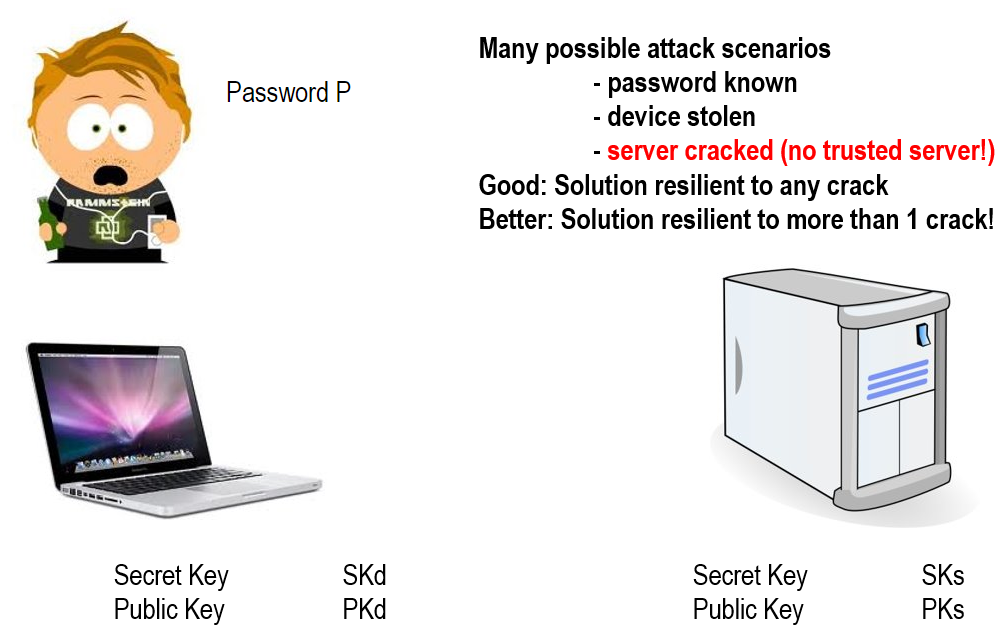
\includegraphics[scale=0.5]{2022-01-06-16-43-18.png}% chktex 8
\end{figure*}
\subsection{Basic Solution}
La soluzione base risolve tutte le combinazioni di attacchi precedenti tranne una in cui bisogna applicare tecniche più avanzate.
\subsubsection{Tickets}
\begin{itemize}
	\item Assunzioni: il dispositivo deve essere connesso in rete;
	\item Protection: cifra la chiave del dispositivo cosicché possa essere decifrata solamente con la cooperazione del server;
	\item Idea: \begin{enumerate}
		      \item Invia il ticket cifrato al server (contiene dati per autenticare l'utente e non si ha bisogno che siano salvati);
		      \item Usa il contenuto del ticket per autenticare l'utente:
		      \item Usa il contenuto del ticket per decifrare parzialmente la chiave del dispositivo.
	      \end{enumerate}
\end{itemize}
\subsubsection{Protocol Inizialization}
\begin{figure*}[h]
	\centering
	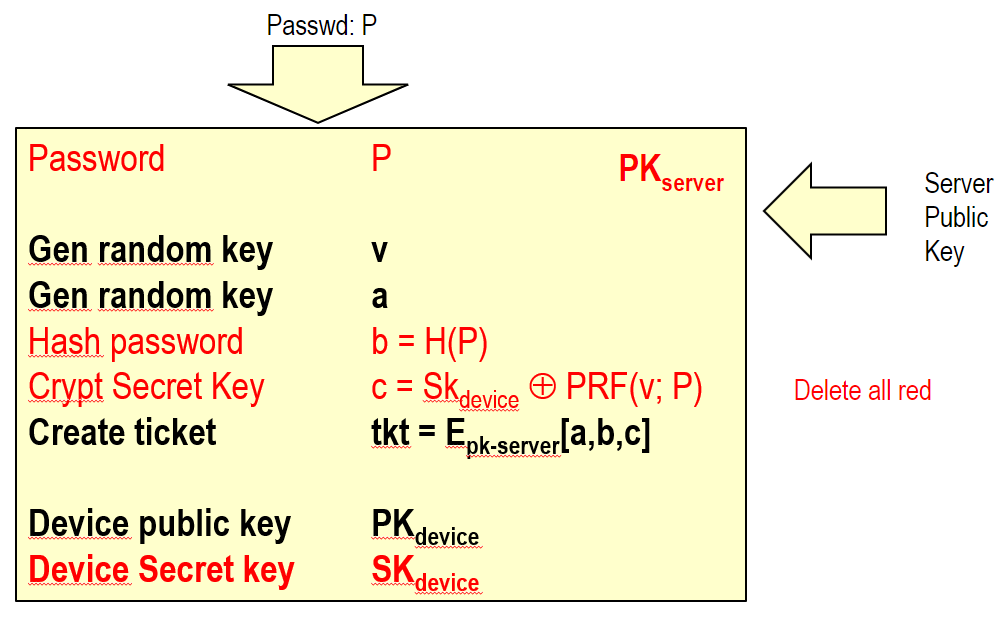
\includegraphics[scale=0.5]{2022-01-06-16-51-03.png}% chktex 8
\end{figure*}
Il tempo in cui registriamo il dispositivo inseriamo la vera \textcolor{red}{password P} e salvata temporaneamente nel dispositivo\@.Sappiamo la chiave \textcolor{red}{pubblica del serve \(PK_{server}\)} e quella \textcolor{red}{pubblica \(PK_{device}\) e privata \(SK_{device}\) del dispositivo}\@.
\begin{itemize}
	\item generiamo due chiavi casuali \(v,a\);
	\item \textcolor{red}{Eseguiamo l'hash della password \(b=H(P)\)};
	\item \textcolor{red}{Cifriamo la chiave segreta \(c=SK_{device}\bigoplus PRF(v,P)\)};
	\item Crea il ticket \(tkt=E_{PK_{server}[a,b,c]}\);
\end{itemize}
\begin{Importante}
	Tutto ciò che è in rosso viene cancellato appena letto.
\end{Importante}
\newpage
\subsubsection{Key Retrival}
\begin{figure*}[h]
	\centering
	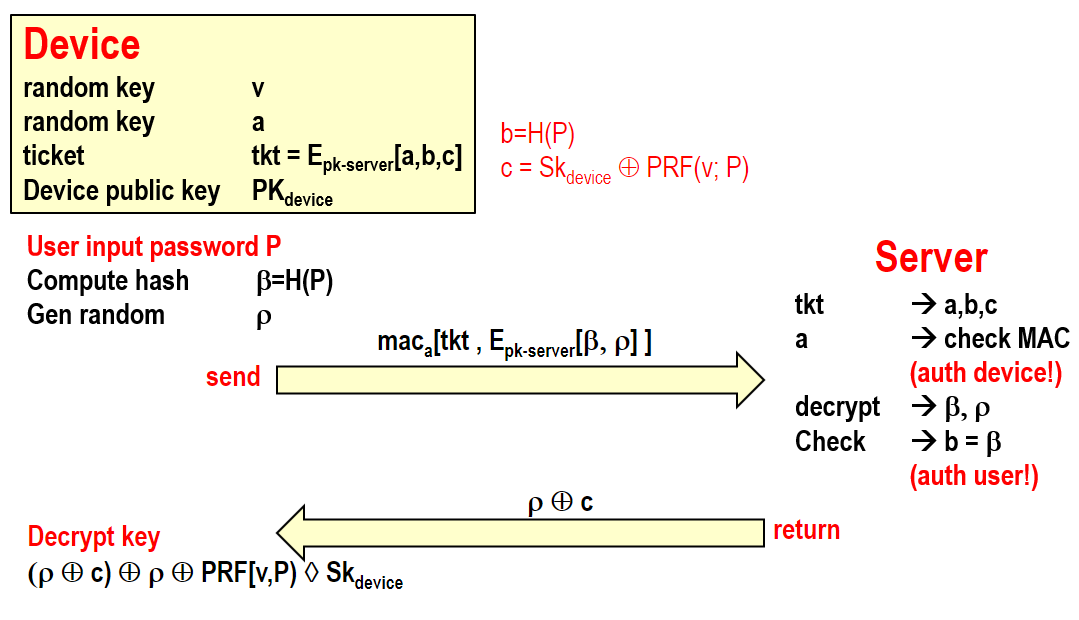
\includegraphics[scale=0.4]{2022-01-06-17-06-20.png}% chktex 8
\end{figure*}
Accedo al dispositivo inserendo la password \(P\) calcolo localmente \(\beta =H(P)\) e genero il valore casuale \(\rho \) \@. Ora invio al server un messaggio che contiene:\begin{itemize}
	\item \(tkt=E_{PK_{server}[a,b,c]}\);
	\item \(E_{PK_{server}}[\beta ,\rho ]\);
\end{itemize}
Autentico questo messaggio tramite HMAC con chiave a.\newline
Ora chiedo assistenza al server:\begin{itemize}
	\item Apro il ticket e prelevo il valore \(a\);
	\item Verifico che il messaggio è stato inviato effettivamente da quel dispositivo controllando il MAC\@;
	\item Decrypt l'hash della password \(\beta ,\rho \);
	\item Controllo che la password originale sia uguale a quella ricevuta \(\beta = b\);
	\item \textcolor{red}{Ora so che l'utente e il device sono reali};
	\item Il server ritorna \(p\bigoplus s\);
\end{itemize}
Il dispositivo decifra la chiave \((\rho \bigoplus c)\bigoplus \rho \bigoplus PRF(v,P)=SK_{device}\) avendo così il dispositivo autorizzato.
\subsubsection{Attacchi}
Con lo schema appena proposto ci siamo protetti da qualsiasi tipo di attacco eccetto uno (\emph{device stolen and password known}).\begin{itemize}
	\item \textbf{Server cracked e password nota}:\begin{enumerate}
		      \item Se la chiave \(v\) nel dispositivo è ancora segreta allora non asi può ottenere SK poiché cifrata con PRF (v,P)
	      \end{enumerate}
	\item \textbf{Device cracked/stolen}:\begin{enumerate}
		      \item L'attacker deve inviare un hash di una password valida;
		      \item L'attacker può effettuare un dictionary attack online, ma è facilmente rilevabile e il MAC è verificato;
	      \end{enumerate}
	\item \textbf{Device and Server Cracked}:\begin{enumerate}
		      \item Manca solamente la password;
		      \item L'attacker può effettuare un dictionary attack online.
	      \end{enumerate}
\end{itemize}
Per risolvere tutti i problemi fino ad ora proposti si utilizza il secret sharing nella seguente maniera.
\newpage
\subsection{Advanced Solution}
\subsubsection{Secret Sharing (2,2) for RSA}
\begin{figure*}[h]
	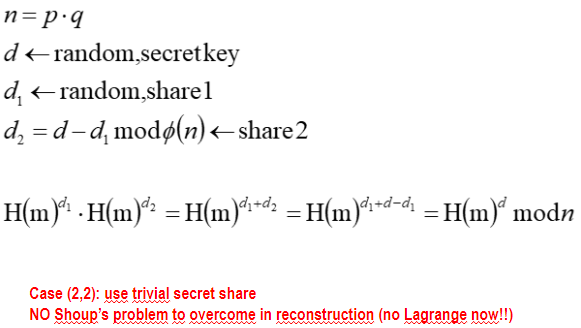
\includegraphics[scale=0.5]{2022-01-06-17-30-36.png}% chktex 8
\end{figure*}
\begin{tabular}{ccc}
	\textbf{Protocol Initialization} & 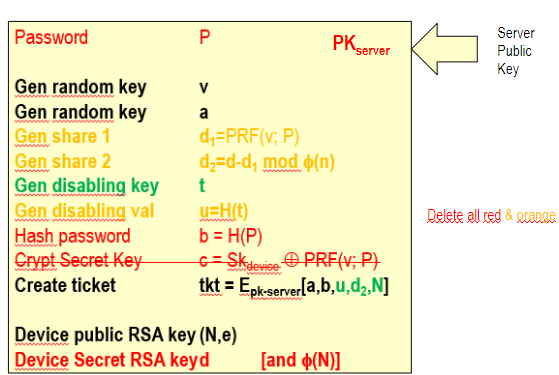
\includegraphics[scale=0.4]{2022-01-06-17-31-58.png} % chktex 8
	                                 &                                                      \\
	\textbf{Key Retrieval}
	                                 & 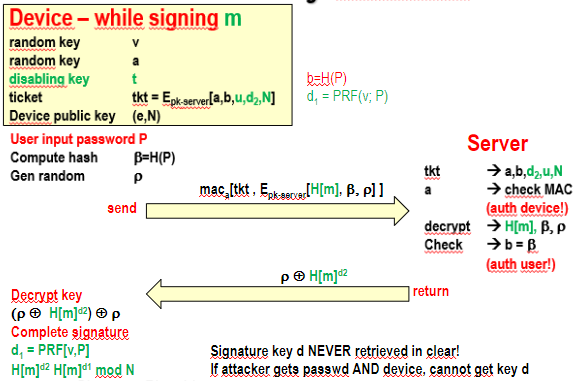
\includegraphics[scale=0.5]{2022-01-06-17-33-30.png} % chktex 8
	                                 &
	\\\textbf{Key Disabling}&
	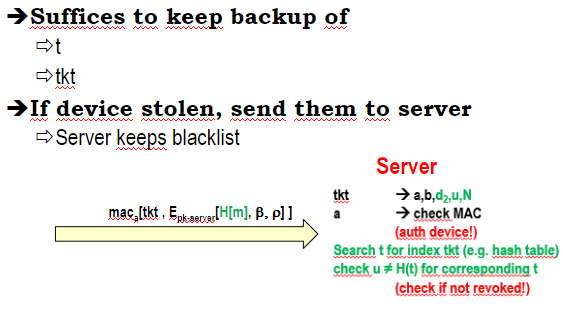
\includegraphics[scale=0.5]{2022-01-06-17-34-40.png}% chktex 8
	                                 &
\end{tabular}
\chapter{Linear Secret Sharing \& Access Control Matrix}
Vogliamo generalizzare il secret sharing in modo tale che, al posto di avere threshold, abbiamo una policy arbitraria.
\section{Revisiting Shamir Scheme}
\begin{itemize}
	\item Segreto \(s\);
	\item Share \(i\): \begin{equation*}
		      y_{i}=s+a_{1}x_{1}+a_{2}x_{i}^{2}+\cdots +a_{t-2}x_{i}^{t-2}+a_{t-1}x_{i}^{t-1}
	      \end{equation*}
	\item In forma vettoriale: prodotto scalare\begin{equation*}
		      y_{i}=[1,x_{i},x_{i}^2,\ldots ,x_{i}^{t-2},x_{i}^{t-1}]\bullet [s,a_{1},a_{2},\ldots ,a_{t-2},a_{t-1}]
	      \end{equation*}
	\item I coefficienti \(a_{{i}}\) sono casuali, rinominiamoli come:\begin{equation*}
		      y_{i}=[1,x_{i},x_{i}^2,\ldots ,x_{i}^{t-2},x_{i}^{t-1}]\bullet [s,r_{1},r_{2},\ldots ,r_{t-2},r_{t-1}]
	      \end{equation*}
\end{itemize}
\subsection{Shamir Scheme in Matrix Form}
\begin{equation*}
	\centering
	Ax=b
\end{equation*}
\begin{itemize}
	\item \(A\) è una matrice \(n\times t\) data;
	\item \(x\) è un vettore di dimensione \(t\) formato da \([secret,rand,rand],.\ldots \);
	\item \(b\) è un vettore di dimensione \(n\) formato dagli shares risultanti.
\end{itemize}
\begin{esempio}
	Schema Shamir in forma matriciale \(3,4\):\begin{equation*}
		\begin{bmatrix}
			1 & x_{1} & x_{1}^2 \\
			1 & x_{2} & x_{2}^2 \\
			1 & x_{3} & x_{3}^2 \\
			1 & x_{4} & x_{4}^2
		\end{bmatrix}
		\begin{bmatrix}
			s \\r_{1}\\r_{2}
		\end{bmatrix}=\begin{bmatrix}
			y_{1} \\y_{2}\\y_{3}\\y_{4}
		\end{bmatrix}
	\end{equation*}
	Matrice \textbf{Vandermonde}
\end{esempio}
\subsubsection{Ricostruzione del segreto}
\begin{itemize}
	\item Sistema lineare t righe, schema per esempio (3,4):\begin{equation*}
		      \begin{bmatrix}
			      1 & x_{1} & x_{1}^{2} \\
			      1 & x_{2} & x_{2}^{2} \\
			      1 & x_{4} & x_{4}^{2}
		      \end{bmatrix}\begin{bmatrix}
			      s \\r_{1}\\r_{2}
		      \end{bmatrix}=\begin{bmatrix}
			      y_{1} \\y_{2}\\y_{4}
		      \end{bmatrix}
	      \end{equation*}
	\item L'incognita è il vettore:\begin{equation*}
		      \begin{bmatrix}
			      s \\r_{1}\\r_{2}
		      \end{bmatrix}
	      \end{equation*}
\end{itemize}
Detto ciò, dato che è un sistema lineare, non abbiamo bisogno di utilizzare l'interpolazione di Lagrange ma possiamo semplicemente:\begin{equation*}
	\begin{bmatrix}
		s \\r_{1}\\r_{2}
	\end{bmatrix}={\begin{bmatrix}
		1 & x_{1} & x_{1}^{2} \\
		1 & x_{2} & x_{2}^{2} \\
		1 & x_{4} & x_{4}^{2}
	\end{bmatrix}}^{-1}\begin{bmatrix}
		y_{1} \\y_{2}\\y_{4}
	\end{bmatrix}
\end{equation*}
La cui inversa vale:\begin{equation*}
	{\begin{bmatrix}
			1 & x_{1} & x_{1}^{2} \\
			1 & x_{2} & x_{2}^{2} \\
			1 & x_{4} & x_{4}^{2}
		\end{bmatrix}}^{-1}=\begin{bmatrix}
		\frac{x_{2}x_{4}}{(x_{1}-x_{2})(x_{1}-x_{4})}
		       & \frac{x_{1}x_{4}}{(x_{2}-x_{1})(x_{2}-x_{4})}
		       & \frac{x_{1}x_{2}}{(x_{4}-x_{1})(x_{4}-x_{2})}          \\
		\cdots & \cdots                                        & \cdots \\
		\cdots & \cdots                                        & \cdots
	\end{bmatrix}
\end{equation*}
I cui elementi sono i coefficienti di Lagrange che, moltiplicati con il vettore \(b\) si ottiene il segreto:\begin{equation*}
	s=y_{1}\frac{x_{2}x_{4}}{(x_{1}-x_{2})(x_{1}-x_{4})}+y_{2}\frac{x_{1}x_{4}}{(x_{2}-x_{1})(x_{2}-x_{4})}+y_{3} \frac{x_{1}x_{2}}{(x_{4}-x_{1})(x_{4}-x_{2})}
\end{equation*}
\subsubsection{Ricostruzione del segreto:alternativa}
\begin{figure*}[h]
	\centering
	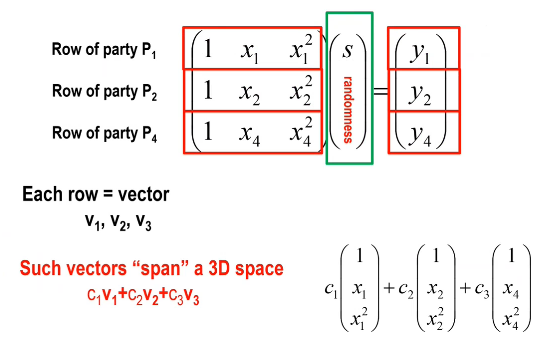
\includegraphics[scale=0.5]{2022-01-07-12-25-58.png}% chktex 8
\end{figure*}
I vettori \(v_{1},v_{2},v_{3}\) devono essere basi dello spazio vettoriale, se così non fosse non si potrebbe ricostruire il segreto poiché la loro combinazione lineare non fornisce tutto lo spazio\@.\newline Quindi, si può ricostruire il segreto se è possibile ricostruire il segreto se esiste una combinazione lineare tra i vettori \(v_{1},v_{2},v_{3}\) pari a \((1,0,0)\):\begin{equation*}
	c_{1}\begin{bmatrix}
		1 & x_{1} & x_{1}^2
	\end{bmatrix}+c_{2}\begin{bmatrix}
		1 & x_{2} & x_{2}^{2}
	\end{bmatrix}+c_{3}\begin{bmatrix}
		1 & x_{4} & x_{4}^{2}
	\end{bmatrix}=\begin{bmatrix}
		1 & 0 & 0
	\end{bmatrix}
\end{equation*}
In forma matriciale:\begin{equation*}
    \begin{bmatrix}
        1&1&1\\x_{1}&x_{2}&x_{3}\\x_{1}^{2}&x_{2}^{2}&x_{3}^{2}
    \end{bmatrix}\begin{bmatrix}
        c_{1}\\c_{2}\\c_{3}
    \end{bmatrix}=\begin{bmatrix}
        1\\0\\0
    \end{bmatrix}
\end{equation*}
Che la sua risoluzione ci porta a:\begin{equation*}
    c_{1}=\frac{x_{2}x_{4}}{(x_{1}-x_{2})(x_{1}-x_{4})};\quad  c_{2}=\frac{x_{1}x_{4}}{(x_{2}-x_{1})(x_{2}-x_{4})};\quad c_{3}=\frac{x_{1}x_{2}}{(x_{4}-x_{1})(x_{4}-x_{2})};
\end{equation*}
Questi coefficienti rispettano la combinazione lineare e quindi:\begin{equation*}
    \{c_{1}\begin{bmatrix}
		1 & x_{1} & x_{1}^2
	\end{bmatrix}+c_{2}\begin{bmatrix}
		1 & x_{2} & x_{2}^{2}
	\end{bmatrix}+c_{3}\begin{bmatrix}
		1 & x_{4} & x_{4}^{2}
	\end{bmatrix}\}\begin{bmatrix}
        s\\r_{1}\\r_{2}
    \end{bmatrix}=\begin{bmatrix}
        1&0&0
    \end{bmatrix}\begin{bmatrix}
        s\\r_{1}\\r_{2}
    \end{bmatrix}=s
\end{equation*}
Quindi, siamo riusciti a trasformare il problema di shamir in un problema di span.
\section{Generalizzazione}
Nel \textbf{Linear Secret Sharing Scheme (LSSS)} è una generalizzazione dello span problem in cui la matrice A è arbitraria.
\subsection{Trivial Secret Share is LSSS}
\begin{esempio}
    Schema \((3,3)\)
    \begin{equation*}
        \begin{bmatrix}
            1&-1&-1\\0&1&0\\0&0&1
        \end{bmatrix}\begin{bmatrix}
            s\\r_{1}\\r_{2}
        \end{bmatrix}=\begin{bmatrix}
            s-r_{1}-r_{2}\\r_{1}\\r_{2}
        \end{bmatrix}
    \end{equation*}
\end{esempio}
\begin{esempio}
    Schema \((3,3)\) Span program
    \begin{equation*}
        c_{1}\begin{bmatrix}
            1&-1&0
        \end{bmatrix}+c_{2}\begin{bmatrix}
            0&1&0
        \end{bmatrix}+c_{3}\begin{bmatrix}
            0&0&1
        \end{bmatrix}=\begin{bmatrix}
            1&0&0
        \end{bmatrix}
    \end{equation*}
    \begin{equation*}
        c_{1}=c_{2}=c_{3}=1
    \end{equation*}
    Ricostruzione del segreto:\begin{equation*}
        c_{1}(s-r_{1}-r_{2})+c_{2}r_{1}+c_{3}r_{2}=(s-r_{1}-r_{2})+r_{1}+r_{2}=s
    \end{equation*}
\end{esempio}
\begin{theorem}[LSSS-homomorphic]
    Qualsiasi LSSS (Linear Secret Sharing Scheme) è \textbf{homomorphic}.
    \begin{proof}
        Supponiamo di avere:\begin{equation*}
            x_{a}=(s_{a},r_{1a},r_{2a},\ldots)\quad y_{a}=(share_{1a},share_{2a},\ldots)
        \end{equation*}
        \begin{equation*}
            x_{b}=(s_{b},r_{1b},r_{2b},\ldots)\quad y_{b}=(share_{1b},share_{2b},\ldots)
        \end{equation*}
        \begin{equation*}
            Ax_{a}=y{a}\quad Ax_{b}=y_{b}
        \end{equation*}
        \begin{equation*}
            y_{a}+y_{b}=Ax_{a}+Ax_{b}=A(x_{a}+x_{b})=A(s_{a}+s_{b},rand,rand,\ldots)
        \end{equation*}
    \end{proof}
\end{theorem}
\subsection{Monotone Span Programs}
Le operazioni fatte fino ad ora, le operazioni sono legate al campo vettoriale in cui si opera\@.Proviamo ad eseguire uno Span Program in GF2 (si può avere o 0 o 1): il segreto è un bit e la sua probabilità di essere indovinato è del 50. Facciamo un esempio in GF2.
\begin{esempio}
\begin{itemize}
    \item 5 parties;
    \item Vettori 4-dimensionali;
    \item La seconda parte ha 2 vettori;
\end{itemize}
\begin{figure*}[h]
    \centering
    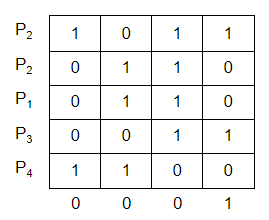
\includegraphics[scale=0.5]{2022-01-08-15-15-29.png}% chktex 8
\end{figure*}
Vogliamo capire se una qualche combinazione lineare di questi vettori ci porta al valore \(\begin{bmatrix}
    1&0&0&0
\end{bmatrix}\) e quindi capace di farmi ricostruire il segreto\@. Quindi, il programma accetta un insieme \(B\) se e solo se lo span delle righe assegnate a \(B\) consentono di arrivare al vettore \(\begin{bmatrix}
    1&0&0&0
\end{bmatrix}\) \@.
Supponiamo che \( \{P_{2},P_{4}\} \) si mettono insieme
\setlength\intextsep{0pt}
\begin{figure*}[h]
	\centering
	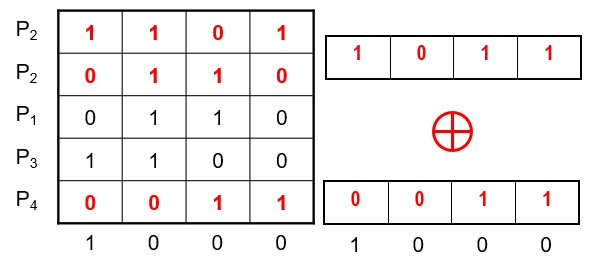
\includegraphics[scale=0.4]{2022-01-08-15-24-44.png}% chktex 8
\end{figure*}
\end{esempio}
e sommo i 3 vettori, ottengo il vettore che cercavamo quindi posso ricostruire il segreto\@.\newline
Supponiamo ora che si uniscano \(P_{1},P_{2}\), non è possibile ricostruire il segreto poiché lo span di questi vettori non ritorna il vettore \(\begin{bmatrix}
    1&0&0
\end{bmatrix}\)
\begin{figure*}[h]
    \centering
    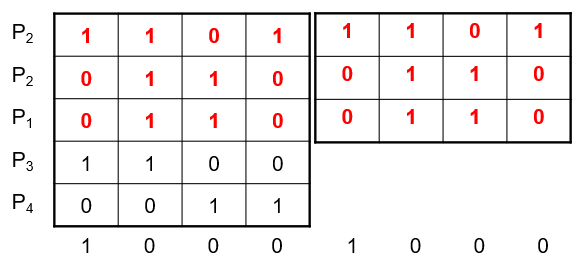
\includegraphics[scale=0.4]{2022-01-08-16-38-44.png}% chktex 8
\end{figure*}
\newpage
\begin{esempio}
    Span Programs\(\rightarrow \)Secret Sharing
    \begin{figure*}[h]
        \centering
        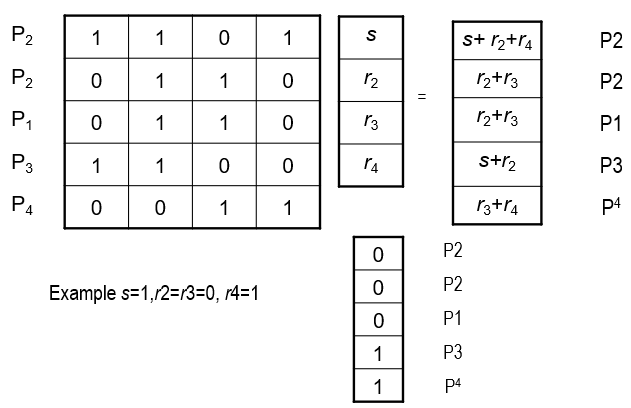
\includegraphics[scale=0.4]{2022-01-08-17-18-40.png}% chktex 8
    \end{figure*}
    \begin{Importante}
        Abbiamo effettuato la moltiplicazione fra le due matrici per ottenere il termine di destra.
    \end{Importante}
\end{esempio}
\subsection{LSSS and Access Structure}
Ogni struttura di accesso monotona può essere implementata con questo schema:\begin{itemize}
    \item Partecipanti \(P= \{P_{1},P_{2},P_{3},P_{4}\} \);
    \item Struttura monotona di accesso: \(A\subseteq 2^{P}\);
\end{itemize}
\begin{Definizione}[Struttura di accesso monotona]
    Una \textbf{struttura di accesso monotona} è una struttura in cui non sono presenti negazioni:\@si ottiene la condizione verificata solo se non vi sono presenti negazioni nella policy implementata.
\end{Definizione}
\begin{esempio}
    \begin{equation*}
        A=\{ \{P_{1},P_{2} \} , \{P_{1},P_{3},P_{4} \} \}
    \end{equation*}
    Con questa notazione, si accede al segreto solo se si coordinano \( \{P_{1},P_{2} \} \) o \( \{P_{1},P_{3},P_{4} \} \) \emph{(Come si può vedere non vi sono negazioni)}
\end{esempio}
Ogni predicato booleano (AND o OR) si può implementare un LSSS che supporta quel determinato predicato\@. Tuttavia, non vi è una regola precisa di implementare un predicato:\@in base a come viene scritta la logica si ha uno schema ideale o meno\@.
\subsubsection{LSSS matrix frmo AC Predicate}
\setlength\intextsep{0pt}
\begin{wrapfigure}[6]{R}[0pt]{0pt}
	\centering
    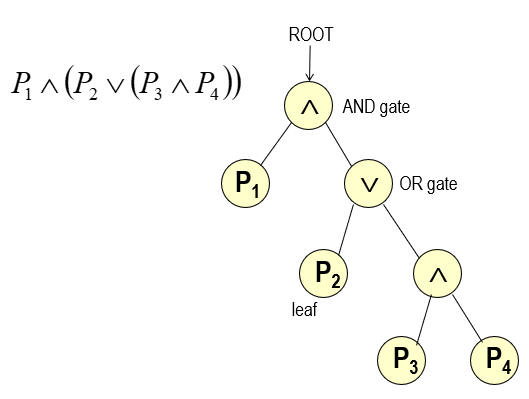
\includegraphics[scale=0.4]{2022-01-08-17-38-41.png}% chktex 8
\end{wrapfigure}
Vogliamo ottenere il segreto se la condizione \(P_{1}\wedge P_{2}\vee (P_{3}\wedge P_{4})\) è verificata e lo vogliamo implementare secondo uno schema di Secret Sharing\@. Scriviamo la policy come un albero:
\begin{enumerate}
    \item Radice;
    \item Da sinistra a destra esegui:\begin{itemize}
        \item Ogni parte \(P_{i}\) rappresenta la foglia dell'albero;
        \item Gli operatori sono i nodi interni dell'albero;
        \item Ogni operatore OR o AND collega la foglia all'albero;
    \end{itemize}
\end{enumerate}
Qual è la matrice che implementa questa policy? A tale scopo, procediamo preliminarmente ad analizzare le singole operazioni\@.
\paragraph{AND Gate}
\setlength\intextsep{0pt}
\begin{wrapfigure}[3]{R}[0pt]{0pt}
	\centering
    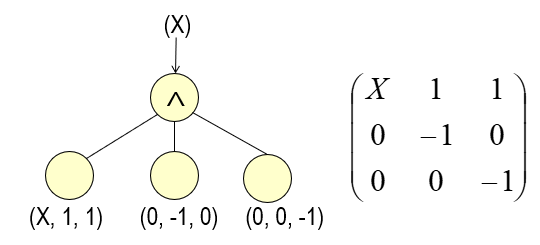
\includegraphics[scale=0.4]{2022-01-08-17-49-09.png}% chktex 8
\end{wrapfigure}
Supponiamo che \(X\) sia il segreto che vogliamo dividere in 3 parti in modo tale che il segreto venga ricostruito solo se tutti e tre condividono il proprio share: (3,3) Trivial Secret Scheme.
\bigskip \bigskip
\begin{Importante}
    La matrice \(\begin{bmatrix}
        X&1&1\\0&1&0\\0&0&-1
    \end{bmatrix}\) viene ottenuta tenendo conto che le righe sono le parties e che lo span (combinazione lineare) delle righe debba ritornare \(\begin{bmatrix}
        1&0&0
    \end{bmatrix}\) (X,0,0)\@. Quindi era valida anche la seguente matrice:\begin{equation*}
        \begin{bmatrix}
            X&-1&1\\0&1&0\\0&0&1
        \end{bmatrix}\quad \text{\textbf{Relativi Pesi:}}\quad c_{1}=1,c_{2}=1,c_{3}=-1
    \end{equation*}
    Infatti:\begin{equation*}
        c_{1}P_{1}+c_{2}P_{2}+c_{3}P_{3}=1\begin{bmatrix}
            X&-1&1
        \end{bmatrix}+1\begin{bmatrix}
            0&1&0
        \end{bmatrix}-1\begin{bmatrix}
            0&0&1
        \end{bmatrix}=\begin{bmatrix}
            X&0&0
        \end{bmatrix}
    \end{equation*}
\end{Importante}
\medskip
\paragraph{OR Gate}
\setlength\intextsep{0pt}
\begin{wrapfigure}[3]{R}[0pt]{0pt}
	\centering
    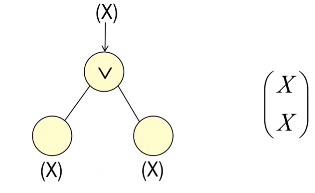
\includegraphics[scale=0.4]{2022-01-08-18-06-14.png}% chktex 8
\end{wrapfigure}
Sia \(X\) il segreto che stiamo condividendo a due parties\@.La condizione OR ci dice che per ricostruire il segreto, deve essere presente una delle due parti\@.\newline
Quindi possiamo modellare la matrice come \(\begin{bmatrix}
    X\\X
\end{bmatrix}\).
\medskip
\paragraph{Ricostruzione della matrice}
La condizione era \(P_{1}\wedge P_{2}\vee (P_{3}\wedge P_{4})\) \@.\newline \bigskip
\begin{figure*}[th]
    \begin{tabular}{cc}
        \begin{minipage}{0.45\textwidth}
            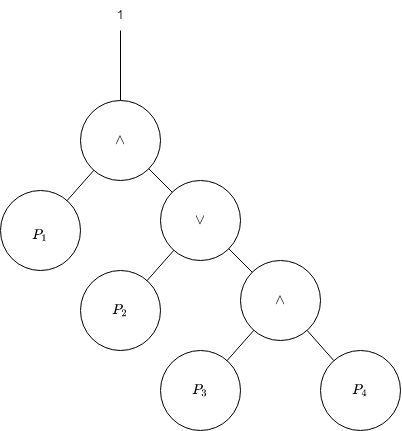
\includegraphics[scale=0.4]{first.png}
            \captionof{figure}{Fase 1:\@assumiamo il segreto di una dimensione e quest'ultimo deve essere diviso in due per essere ricostruito.}
        \end{minipage}
            &\begin{minipage}{0.45\textwidth}
                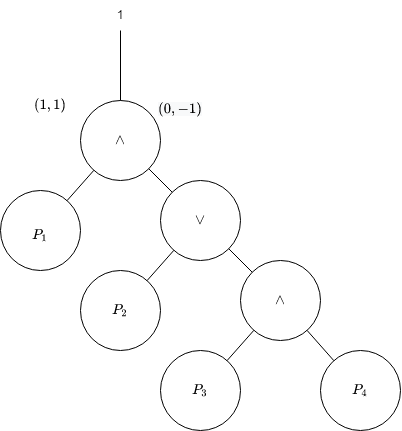
\includegraphics[scale=0.4]{second.png}
                \captionof{figure}{Fase 2: Calcolo gli shares necessari e li spartisco nei rami \(P_{1}\rightarrow (1,1)\) e \(\wedge \rightarrow (0,-1)\)}
            \end{minipage}\\
            \begin{minipage}{0.45\textwidth}
                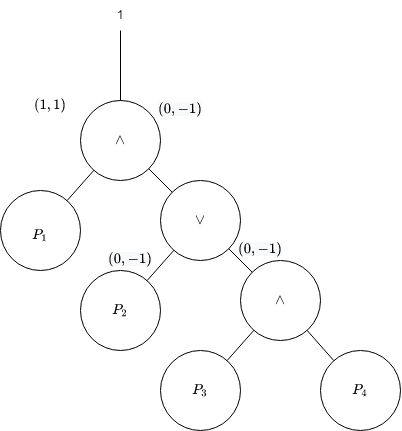
\includegraphics[scale=0.4]{third.png}
                \captionof{figure}{Fase 3: dato che non so se ci sono delle parti o meno prendo lo share e lo copio in entrambi i rami \textbf{poiché uno dei due deve conoscere il segreto per risalire l'albero}.}
            \end{minipage}
            &
            \begin{minipage}{0.45\textwidth}
                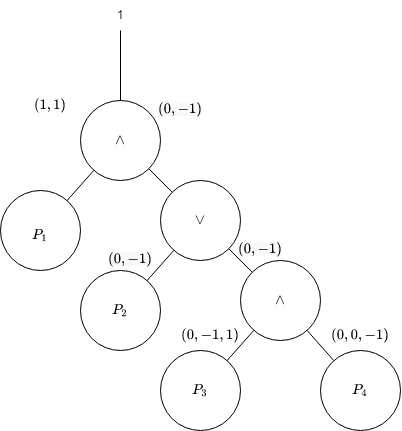
\includegraphics[scale=0.4]{fourth.png}
                \captionof{figure}{Fase 4: Mi trovo di fronte ad un AND e quindi il segreto deve essere conosciuto da entrambi. Aumentiamo la dimensione del vettore e generiamo due valori consoni per ottenere il valore del padre cioè \((0,-1)\), come nella fase 1 si è scelto 1 e -1}
            \end{minipage}
    \end{tabular}
\end{figure*}
Quello che manca ora è di riassumere tutti i vettori che sono stati assegnati durante la ricostruzione della matrice:\begin{equation*}
    \begin{matrix}
        P_{1}:\begin{bmatrix}
            1&1&0
        \end{bmatrix}\\
        P_{2}:\begin{bmatrix}
            0&-1&0
        \end{bmatrix}\\
        P_{3}:\begin{bmatrix}
            0&-1&1
        \end{bmatrix}\\
        P_{4}:\begin{bmatrix}
            0&0&-1
        \end{bmatrix}\\
    \end{matrix}
\end{equation*}
Per effettuare le verifiche si pone ad uno la/le parties che dovrebbero contribuire a ricostruire il segreto, si effettuano le somme e non si deve ottenere il vettore \(\begin{bmatrix}
    1&0&0
\end{bmatrix}\).
\newpage
\begin{esempio}[Esercizio]
    Verifica che la policy proposta rispetta la condizione data:
    \begin{figure*}[h]
        \centering
        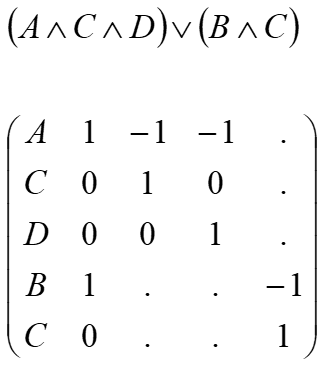
\includegraphics[scale=0.4]{2022-01-08-19-34-43.png}% chktex 8
    \end{figure*}
\end{esempio}
\section{Conclusione}
\begin{figure*}[th]
    \centering
    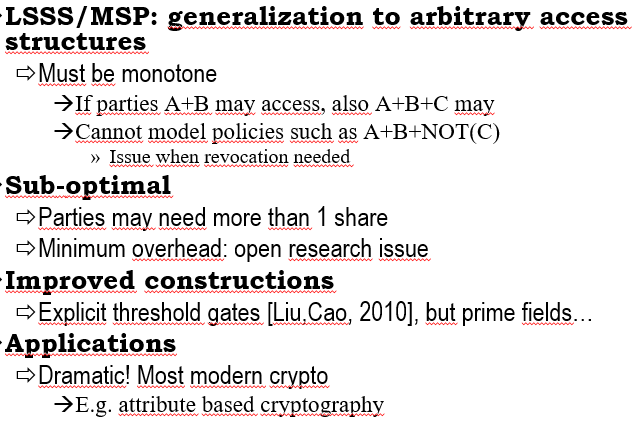
\includegraphics[scale=1]{2022-01-08-19-39-12.png}% chktex 8
\end{figure*}
\chapter{Elliptic Curve Crypto}
\section{Introduction}
La public key cryptography si basa sul fatto di rendere una operazione facile in un verso, ma difficile nell'altro. Questo concetto viene detto \textbf{computational security}\@.\newline
Le curve ellittiche servono ad ottenere computational security anche in assenza di operazioni con modulo:\@invece del modulo si utilizza il DLog. La complessità per invertire l'operazione del DLOG in \(Z^{*}(p)\) è \(\exp{(O^{\frac{1}{3}})}\); nel caso in cui si cambia il gruppo in \((Z(p),+)\) è polinomiale infatti:\begin{itemize}
	\item \(Z(p)\) è l'insieme dei numeri \( \{0,\ldots ,p-1 \} \);
	\item \(+\) è la somma \(\mod{p}\) i.e.\(3+9\mod{11}=1\);
	\item è un gruppo abeliano poiché soddisfa tutte le proprietà dei gruppi e quella di essere abeliano;
	\item Supponiamo che la moltiplicazione venga espressa come somma di \(k\) volte e che ci venga dato il risultato i.e.\(k\cdot 3\mod{p}=result\);
	\item Il corrispondente \textbf{Discrete Log Problem (DLOG)} consiste nel trovare \(k\) tale che \(k\cdot 3\mod{p}=result\); \emph{(nel caso si abbia una moltiplicazione si ha \(g^{x}\))};
	\item Quindi questo problema è risolvibile polinomialmente tramite un algoritmo.
\end{itemize}
Dato che questo in questo gruppo, il problema è risolvibile polinomialmente e quindi in maniera facile non è adatto nella crittografia. Tuttavia, si introduce un problema più difficile nei \textbf{gruppi delle curve ellittiche} con difficoltà computazionale \(\exp{(O^{\frac{1}{2}})}\) (\emph{Polland Rho}).
La vera convenienza delle curve ellittiche è per la sua \textbf{scalabilità}.
\section{Elliptic Curves}
\begin{Definizione}[Curve Ellittiche]
	Una \textbf{curve ellittica} è una particolare curva cubica di terzo ordine che, nella sua forma più generale (\emph{Weierstrass Expression}) ha questa struttura:\begin{equation*}
		\centering
		y^{2}=x^{3}+ax+b\quad where \quad 4a^{3}+27b^{2}\neq 0
	\end{equation*}
\end{Definizione}
Per avere un gruppo dobbiamo avere un insieme di curve e una operazione che è chiusa rispetto all'insieme. Questa operazione è \(+\) o anche detta \(\circ \): tale che \(P+Q=R\) con \(R\) appartenente alla curva.\newpage
\section{Elliptic point addition \(P+Q\)}
Per definire l'operazione di addizione si seguono i seguenti passi:
\begin{figure*}[th]
    \begin{tabular}{cc}
        \begin{minipage}{0.45\textwidth}
            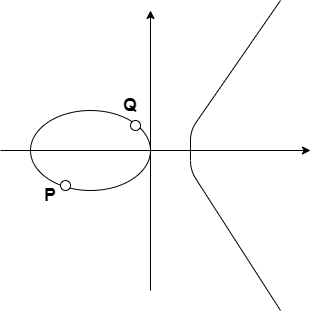
\includegraphics[scale=0.4]{ECaddition.png}
            \captionof{figure}{Prendiamo due punti (per ora distinti appartenenti alla curva ellittica)}
        \end{minipage}
            &\begin{minipage}{0.45\textwidth}
                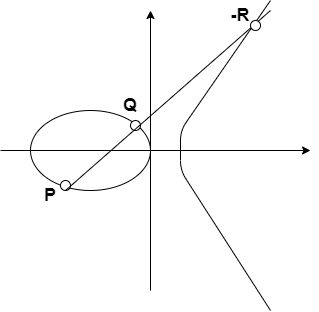
\includegraphics[scale=0.4]{ECaddition2.png}
                \captionof{figure}{Tracciamo una retta passanti per i due punti e, dato che la curva è cubica, la retta intersecherà la curva ellittica in un altro punto chiamato -R}
            \end{minipage}\\
            \begin{minipage}{0.45\textwidth}
                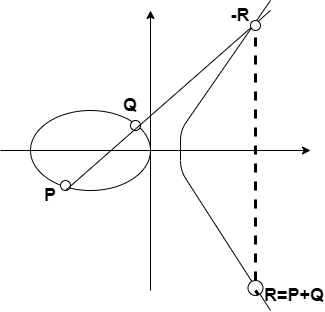
\includegraphics[scale=0.4]{ECaddition3.png}
                \captionof{figure}{Tracciamo il negativo di R che intersecherà la curva ellittica in R. Questo punto lo definiamo \textbf{R=P+Q}}
            \end{minipage}
    \end{tabular}
\end{figure*}
Per verificare la validità di questa operazione dobbiamo verificare le proprietà di gruppo:\begin{itemize}
	\item \textbf{Chiusura}:\@presi due elementi \(g_{1},g_{2}\) del gruppo, allora \(g_{x}=g_{1}\circ g_{2}\) deve appartenere al gruppo;
	\item \textbf{Identità}:\@deve esiste un membro del gruppo tale che \(g\circ I = I\circ g=g\);
	\item \textbf{Inversa}:\@per ogni \(g\) esiste \(g^{-1}\) tale che \(g\circ g^{-1}=I\);
	\item \textbf{Associativa}:\@per qualsiasi \(g_{1},g_{2},g_{3}\) deve valere \((g_{1}\circ g_{2})\circ g_{3}=g_{1}\circ (\circ g_{3})\)
\end{itemize}
\subsection{Elliptic Curves: chiusura}
La chiusura dello operazione rispetto all'insieme non è sempre definita poiché, se prendessimo 2 punti posti verticalmente e li sommiamo come prima, la retta non interseca la curva ellittica. Per ovviare a questo problema introduciamo un punto aggiuntivo detto \textbf{O=-O} che è posto all'infinito.
\begin{Importante}
	Se vogliamo effettuare P+P, introduciamo la tangente alla curva e la sua prossima intersezione la consideriamo come -R.
\end{Importante}\newpage

\subsection{Elliptic Curves: inversa}
\begin{wrapfigure}[10]{R}[0pt]{0pt}
	\centering
	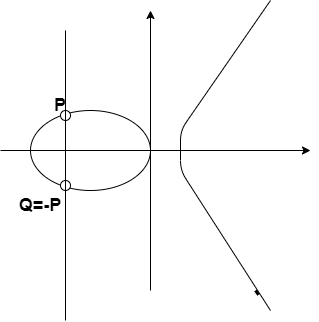
\includegraphics[scale=0.35]{ECaddition4.png}% chktex 8
\end{wrapfigure}
Supponiamo di voler sommare P e -P, il risultato sarà il punto all'infinito \(O=-O\) poiché non si interseca la curva. Dato che \(P-P=0\), possiamo considerarla come l'inversa di P\@.\newline
Essa viene segnata con il -.
\begin{Importante}
	L'inversa viene segnata con il \(-P\) al posto di \(P^{-1}\) poiché nel secondo caso corrisponderebbe all'inversa del gruppo moltiplicativo e non additivo.
\end{Importante}
\begin{Importante}
	\(O=-O\) prende il nome di \(0\quad (zero)\) poiché, se effettuiamo x+0.
	\begin{figure*}[ht]
		\begin{subfigure}[l]{0.4\textwidth}
			\centering
		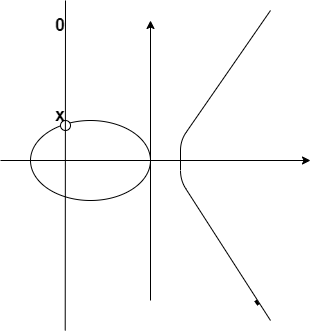
\includegraphics[scale=0.4]{ECaddition5.png}
		\end{subfigure}
		\begin{subfigure}[l]{0.4\textwidth}
			\centering
		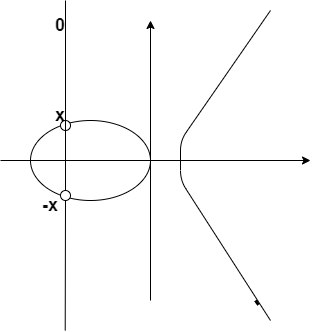
\includegraphics[scale=0.4]{ECaddition6.png}
		\end{subfigure}
	\end{figure*}
	Tracciamo la retta che interseca la curva, segniamo il punto (\emph{in questo caso coincide con x}) e ne prendiamo il suo opposto \(-x\).
\end{Importante}
\subsection{Elliptic Curves:associatività,identità,commutativa}
Queste 3 proprietà sono banalmente verificate.
\begin{theorem}
	Se 3 punti di una curva ellittica appartengono alla stessa linea, allora la loro somma è zero.
	\begin{figure*}[h]
		\centering
		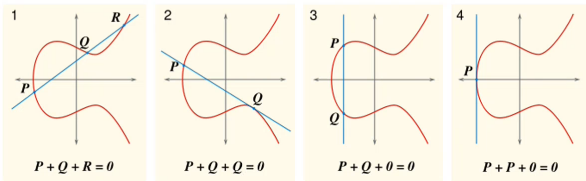
\includegraphics[scale=0.5]{2022-01-11-15-31-30.png}% chktex 8
	\end{figure*}
\end{theorem}
\subsection{Elliptic Curves:Procedura}
Un'altra alternativa di effettuare le operazioni con le curve ellittiche è quella di procedere per via analitica in questo modo:\begin{align*}
	P&=(x_{1},y_{1})\\
	Q&=(x_{2},y_{2})\\
	R&=P+Q=(x_{3},y_{3})\\
	x_{3}&=\lambda^{2}-x_{1}-x_{2}\\
	y_{3}&=\lambda(x_{1}-x_{3})-y_{1}\\
	\lambda&=\begin{cases}
		\frac{y_{2}-y_{1}}{x_{2}-x_{1}} \quad P\neq Q\\
		\frac{3x_{1}^{2}+a}{2y_{1}} \quad P=Q
	\end{cases}
\end{align*}
\newpage
\begin{adjustbox}{valign=C,raise=\strutheight,minipage={1.0\linewidth}}
	\begin{wrapfigure}{r}{0.5\linewidth}
		\centering
		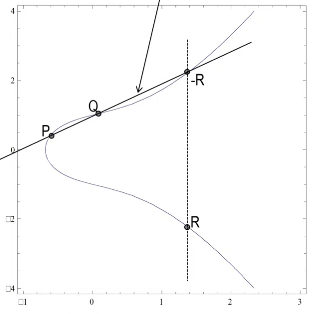
\includegraphics[scale=0.45]{2022-01-11-16-08-52.png}% chktex 8
	\end{wrapfigure}%
	\strut{}
\vspace*{-0.5cm} % This is a fudge to align the top of the theorem environment with the image
	\begin{proof}
		Perché \(P\neq Q\).\newline
		La retta passante tra P e Q è:
		\begin{equation*}
			\centering
			y=y_{1}+\frac{y_{2}-y_{1}}{x_{2}-x_{1}}(x-x_{1})=\lambda(x-x_{1})+y_{1}
		\end{equation*}
			Sostituiamo l'equazione della retta nell'equazione della curva ellittica.
			\begin{flalign*}
				\centering
				y^{2}&=x^{3}+ax+b&\\
				{(\lambda(x-x_{1})+y_{1})}^2&=x^{3}+ax+b&
			\end{flalign*}
		\(\lambda ,x_{1},y_{1}\) sono noti, mentre \(x\) è l'incognita. Non vi è una procedura per risolvere in maniera generica una equazione d terzo grado, ma possiamo ricondurci alle soluzioni poiché sappiamo che i punti della curva sono P e Q. Quindi la soluzione generale è nella forma:\begin{equation*}
			(x-x_{1})(x-x_{2})(x-x_{3})=x^{3}-(x_{1}+x_{2}+x_{3})x^{2}+\cdots
		\end{equation*}
		La cui incognita è \(x^{3}\) e il termine \((x_{1}+x_{2}+x_{3})\) che è pari a \(\lambda \) (noto) ci porta a risolvere:\begin{equation*}
			\centering
			\lambda^{2}=x_{1}+x_{2}+x_{3}\rightarrow x_{3}=\lambda^{2}-x_{1}-x_{2}
		\end{equation*}
		Per quanto riguarda la \(y_{3}\), viene ottenuta dall'equazione della curva:\begin{equation*}
			y_{3}=\lambda (x_{1}-x_{3})-y_{1}
		\end{equation*}
	\end{proof}%
\end{adjustbox}
\begin{adjustbox}{valign=C,raise=\strutheight,minipage={1.0\linewidth}}
	\begin{wrapfigure}{r}{0.5\linewidth}
		\centering
		\includegraphics[scale=0.45]{2022-01-11-17-33-18.png}% chktex 8
	\end{wrapfigure}%
	\strut{}
\vspace*{-0.5cm} % This is a fudge to align the top of the theorem environment with the image
\begin{proof}
	Perché \(P=Q\).\newline
	Nell'equazione della retta non vi è più il coefficiente angolare, ma la tangente:\begin{flalign*}
		y&=y_{1}+y_{1}'(x-x_{1})+y_{1}&\\
		2y\frac{dy}{dx}&=3x^{2}+a\rightarrow \frac{dy}{dx}=\frac{3x^{2}+a}{27}&\\
		\lambda=y_{1}'=\frac{3x_{1}^{2}+a}{2y_{1}}
	\end{flalign*}
	Il resto prosegue come nel caso \(P\neq Q\).
\end{proof}
\end{adjustbox}
\section{Elliptic Curve Group}
\subsection{Elliptic Curves Modular Integers}
Restringiamo l'uso delle curve ellittiche non a numeri reali, ma fra interi in modulo.
\begin{Definizione}
	Una \textbf{elliptic curves modular integers} è una curva ellittica \(E_{p}(x,y)\) che soddisfa le seguenti condizioni:\begin{itemize}
		\item  \(x,y\) siano numeri interi;
		\item \(y^{2}\mod{p}=x^{3}+ax+b \mod{p}\).
	\end{itemize}
\end{Definizione}
Dato che questo campo è finito, allora il numero di punti della curva è finito\@.\newpage
\begin{adjustbox}{valign=C,raise=\strutheight,minipage={1.0\linewidth}}
	\begin{wrapfigure}{r}{0.5\linewidth}
		\centering
		\includegraphics[scale=0.45]{2022-01-11-18-42-46.png}% chktex 8
	\end{wrapfigure}%
	\strut{}
\vspace*{-0.5cm} % This is a fudge to align the top of the theorem environment with the image
\begin{esempio}
		Curva ellittica \(x^{3}+x+1\mod{5}\)\newline
	Le condizioni da soddisfare sono le seguenti e devono essere soddisfatte da tutti i punti:tutti i punti \((i,j) \)tali che \begin{itemize}
		\item \((i,j)\in [0,4]\);
		\item \(j^{2}=i^{3}+i+1\mod{5}\);
		\item Punto all'infinito
	\end{itemize}
	Quindi:\begin{equation*}
		E(Z_{5})=\{O,(0,1),(0,4),(2,1),(2,4),(3,1),(3,4),(4,2),(4,3)\}
	\end{equation*}
	Supponiamo di prendere un punto come punto iniziale:\begin{flalign*}
		&P=(0,1)&\\
		&P+P=(0,1)+(0,1)&\\
		&\text{Passo 1: calcolare \(\lambda \)}&\\
		&\lambda =\frac{3x_{1}^{2}+a}{2y_{1}}=1\cdot 2^{-1}=1\cdot 3=3\mod{5}&\\
		& \text{\(2^{-1}\mod{5}=2x=1\mod{5}=3\) }&\\
		&\text{Passo 2: calcolare \(x_{3}\)}&\\
		&x_{3}=\lambda^{2}-x_{1}-x_{1}=3^{2}=4\mod{5}&\\
		&\text{Passo 3:calcolare \(y_{3}\)}&\\
		&y_{3}=\lambda (x_{1}-x_{3})-y_{1}=3(0-4)-1=2\mod{5}&\\
		&\text{Risultato:\((4,2)\)}&
	\end{flalign*}
	Iterando:\begin{align*}
		P&=(0,1)\\
		2P&=(0,1)+(0,1)=(4,2)\\
		3P&=(4,2)+(0,1)=(2,1)\\
		4P&=(2,1)+(0,1)=(3,4)\\
		5P&=(3,4)+(0,1)=(3,1)\\
		6P&=(3,1)+(0,1)=(2,4)\\
		7P&=(2,4)+(0,1)=(4,3)\\
		8P&=(4,3)+(0,1)=(0,4)\\
		9P&=(0,4)+(0,1)=O
	\end{align*}
	Notiamo che partendo da P, il gruppo è ciclico.
\end{esempio}
\end{adjustbox}
\subsection{Elliptic Curves Group}
In conclusione, \((E(Z_{p}),+)\) è un gruppo per cui:\begin{enumerate}
	\item L'addizione è chiusa su un insieme \(E\) definita dalla curva ellittica;
	\item L'addizione è commutativa;
	\item O è l'identità;
	\item Ogni punto \(P\in E\) possiede l'inversa \(-P\);
	\item Vale la proprietà associativa;
	\item è un gruppo abeliano;
\end{enumerate}
\subsubsection{Proprietà Elliptic curver group in crypto}
Sia \(P\) un punto della curva ellittica appartenente al gruppo \(Z_{p}\) e \(k\) intero mod group order:
\begin{itemize}
	\item Dato \(P\) e \(k\) è facile calcolare \(k\cdot P\);
	\item Dato \(P\) e \(kP\) è difficile calcolare \(k\);
	\item Questo problema è equivalente al problema del DLog in\(Z_{p}\):se abbiamo la notazione moltiplicativa \(k\rightarrow P^{k}\).
	\item In criptografia si ha una forte dipendenza dalla curva scelta: si estendono questi discorsi oltre che in \(Z_{p}\), ma anche nel campo di Galua.
\end{itemize}
\begin{figure*}[h]
	\centering
	\includegraphics[scale=1]{2022-01-12-11-39-51.png}% chktex 8
\end{figure*}
\chapter{ECDH/ECDSA}
In qualsiasi problema crittografico, si calcola \(g^{x}\mod{p}\) che nelle curve ellittiche corrisponde a moltiplicare \(x\) volte \(g\) punto appartenente al gruppo della curva.
\section{ECDH:Elliptic Curves Diffie-Hellman}
Lo scambio chiavi di Diffie-Hellman con le curve ellittiche funziona esattamente come Diffie-Hellman generale, ma con la differenza che si utilizzare il gruppo delle curve ellittiche. Quindi ECDH è un protocollo di accordo delle chiavi.
\vspace*{0.5cm}
\begin{figure*}[ht]
	\centering
	\includegraphics[scale=0.7]{ECDH.png}
\end{figure*}
\begin{enumerate}
	\item C genera x casuale e calcola \([x]G\) in cui G è una curva ellittica;
	\item Invia \(G,[x]G\);
	\item S genera y casuale e calcola \([y]G\), per la proprietà di gruppo (additiva) può calcolare il segreto \([yx]G\) tramite la conoscenza di \(y\);
	\item Invia \([y]G\);
	\item C calcola il segreto \([xy]G\);
\end{enumerate}
\section{ECDSA}
ECDSA è un protocollo per la firma digitale a modulo di un numero primo da 256 e 384 bit basato sul DLog.
\subsection{DSA}
Nella versione standard di \textbf{DSA} si utilizzano le operazioni modulari in \(Z*(p),p>2\) numero primo e \(q\) strong prime cioè: se p è primo \(p=2q+1\). Inoltre, lo span di \(g^{x}\mod{p}\) comprende tutti gli elementi del gruppo.
\begin{Importante}
	Chiave privata \(d\), chiave pubblica \(y=g^{d}\mod{p}\)
\end{Importante}
Quando si firma, dobbiamo effettuare le seguenti operazioni:\begin{itemize}
	\item Generare un valore casuale \(k\in (1,q)\);
	\item Calcolare \(r=(g^{k}\mod{p})\mod{q}\);
	\item Calcolare \(s=k^{-1}(H((m)+dr))\mod{q}\);
	\item la firma:\((r,s)\);
\end{itemize}
Per verificare la firma, occorre:\begin{itemize}
	\item Calcolare \(u_{1}=s^{-1}H(m)\mod{q}\);
	\item Calcolare \(u_{2}=s^{-1}r\mod{q}\);
	\item Verificare \(((g^{u_{1}}y^{u_{2}})\mod{p})\mod{q}= r\)
	\item \(g^{u_{1}}y^{u_{2}}=g^{u_{1}}g^{d\cdot u_{2}}=g^{k}=M\)
	\item \(u_{1}+d\cdot u_{2}=\frac{H(m)k}{H(m)+rd}+\frac{d\cdot r\cdot k}{H(m)+rd}=k\)
\end{itemize}
\subsubsection{Problematiche}
Nel caso in cui k viene predetto la costruzione porta a dei rischi.Infatti, un attacco che è possibile fare è dovuto all'errore di ottimizzazione nel ricalcolo della curva ellittica in ogni firma:k viene predetto o riutilizzato.
Quindi, k non deve essere predicibile poiché, altrimenti, si può firmare un qualsiasi messaggio casuale, si può rubare la chiave privata e quindi perdere la propria identità digitale\@.In particolare:
\begin{algorithm}[H]
	\caption{K predicted}
	\begin{algorithmic}
		\Ensure{\((r,s),\ k\)}
		\State{\(s=k^{-1}[H(m)+rd]\mod{n}\)}
		\State{\(sk=H(m)+rd\mod{n}\)}
		\State{\([sk-H(m)]r^{-1}=d\mod{n}\)}
		\State{\(d\) viene calcolato}
	\end{algorithmic}
\end{algorithm}
\vspace{0.2cm}
Invece, nel caso in cui si ripete k:
\begin{figure*}[h]
	\centering
	\includegraphics[scale=0.5]{2022-01-14-10-15-00.png}% chktex 8
	\caption{K riutilizzato}
\end{figure*}
\subsection{ECDSA:setup}
In ECDSA, dati:\begin{itemize}
	\item \(E(Z_{p})\) curva ellittica con p numero primo;
	\item \(n\) differente da p e numero grande;
	\item \(P\) generatore del gruppo;
	\item \(Q=[d]P\):\begin{enumerate}
		\item \(d\) è un intero casuale tra \([1,n-1]\) \textbf{chiave privata};
		\item \(Q=dP\) punto sulla curva \(chiave pubblica\).
		\end{enumerate}
\end{itemize}\newpage
\subsection{ECDSA:signature generation}
\begin{algorithm}[H]
	\caption{Signature generation}
	\begin{algorithmic}
		\State{Seleziona casualmente un intero \(k\in [1,n-1]\):\begin{itemize}
			\item unico per ogni firma;
			\item non predicibile;
		\end{itemize}}
		\State{Calcola il puntto sulla curva ellittica \(kP=(x_{1,y_{1}})\)}:\begin{itemize}
			\item \(x_{1}\) è un intero \(\mod{P}\)
		\end{itemize}
		\State{Calcola \(r=x_{1}\mod{n}\) è un numero e non un punto della curva ellittica}
		\State{Calcola \(k^{-1}\mod{n}\)}
		\State{Effettua l'hash del messaggio i.e. SHA}
		\State{Firma:\((r,s)\quad s=k^{-1}(H(m)+dr)\)}
	\end{algorithmic}
\end{algorithm}
\subsection{ECDSA:verification}
\begin{algorithm}
	\caption{Signature verification}
	\begin{algorithmic}
		\Ensure{Ricevo \(m\ (r,s)\) con \(s=k^{-1}(H(m)+dr)\)}
		\State{Prendo il messaggio \(m\) e calcolo \(H(m)\)}
		\State{Prendo \(s=\frac{H(m)+rd}{k}\) e calcolo \(w=s^{-1}\mod{n}=\frac{k}{H(m)+rd}\)}
		\State{Calcola:\begin{itemize}
			\item \(u_{1}=H(m)w\mod{n}\)
			\item \(u_{2}=rw\)
		\end{itemize}}
		\State{Calcola il punto della curva ellttica:\begin{itemize}
			\item \(u_{1}P+u_{2}Q=(x_{0},y_{0})\)
			\item è possibile grazie alla proprietà homomorphic:\begin{equation*}
				u_{1}P+u_{2}Q=u_{1}P+u_{2}dP=(u_{1}+u_{2}d)P=\frac{H(m)k}{H(m)+rd}+\frac{rkd}{H(m)+rd}=\frac{k(H(m)+rd)}{H(m)+rd}=kP
			\end{equation*}
		\end{itemize}}
		\State{Calcola \(v=x_{0}\mod{n}\)}
		\State{verifica che \(v=r\)}
	\end{algorithmic}
\end{algorithm}
\subsection{Considerazioni}
L'operazione più costosa rispetto a quella modulare è quella fatta fra le curve ellittiche poiché dipende da quante operazioni si devono effettuare sulla curva ellittica. Infatti:
\begin{itemize}
	\item una per generare la chiave pubblica Q\@;
	\item calcolare kP\@;
\end{itemize}
Quindi per questo si è tentati di riutilizzare la stessa k perché, così facendo, si abbassa il costo computazionale dovuto all'utilizzo delle curve ellittiche.
\chapter{Bilinear Maps}
Il \textbf{bilinear maps} viene utilizzato nelle tecniche di crittografia dette \textbf{pairing-based crypto}: si hanno molti gruppi i cui punti vengono trasformati in altri gruppi.
\section{Definizioni}
\begin{Definizione}[Bilinear Map]
	Siano \(G_{1},G_{2},G_{t}\) gruppi ciclici dello stesso gruppo. Una \textbf{mappa bilineare} da \(G_{1}\times G_{2}\rightarrow G_{t}\) è una funzione \(e:G_{1}\times G_{2}\rightarrow G_{t}\) tale che per tutti \(u\in G_{1},\ v\in G_{2},\ a,b\in \mathbb{Z}\) valga:\begin{equation*}
		e(u^{a},v^{b})={e(u,v)}^{ab}
	\end{equation*}
\end{Definizione}
\begin{Importante}
	Vengono dette \textbf{pairings} perché associano coppie di elementi di \(G_{1},G_{2}\) con gli elementi di \(G_{t}\).
\end{Importante}
\begin{Definizione}[Admissible Bilinear Map]
	Sia \(e:G_{1}\times G_{2}\rightarrow G_{t}\) e \(g_{1},g_{2}\) generatori di \(G_{1},G_{2}\) rispettivamente. La mappa \(e\) è una \textbf{mappa bilineare ammissibile} se \(e(g_{1},g_{2})\) genera \(G_{t}\) e \(e\) è efficientemente calcolabile.
\end{Definizione}
\section{Relazione tra \(G_{1},G_{2},G_{t}\)}
\begin{itemize}
	\item \(G_{1},G_{2},G_{t}\) sono tutti gruppi isomorphic di un altro gruppo dato che hanno in comune lo stesso gruppo ciclico;
	\item Sono differenti poiché i loro elementi vengono calcolati in maniera differenti;
	\item Di solito, \(G_{1}=G_{2}\);
	\item etc\dots;
\end{itemize}
\section{Decisional Diffie-Hellman}
\begin{Definizione}[Decisional Diffie-Hellman]
	Dati \(g,g^{a},g^{b}\) e \(\alpha = \{g^{ab},g^{random}\} \). Sapendo che è possibile conoscere il valore \(\alpha \) con un coin flip (una tra le due alternative), è possibile distinguere quale sia il valore? (il vero valore di DH o quello casuale)\newline
	Un gruppo soddisfa il Decisional Diffie-Hellman DDH se non è possibile distinguere tra il numero casuale e il vero coefficiente di Diffie-Hellman.
\end{Definizione}
Se siamo in grado di calcolare Diffie-Hellman, allora non si soddisfa DDH e DH ma non vale il contrario.\newline
Questo problema è differente da quello computazionale di DH.A tale scopo, supponiamo che stiamo affrontando questo problema con ECDDH:\begin{itemize}
	\item Dati \(G,G^{a},G^{b}\) con bilinear pairing:\begin{equation*}
		e(g^{a},g^{b})={e(g,g)}^{ab}
	\end{equation*} (in modulo);
	\item Obiettivo: rompere DDH
\end{itemize}
Il pairing non ci consente, di norma, di calcolare il termine \(g^{ab}\) poiché è una operazione della curva ellittica, ma trasforma i punti in altri. Quindi, non si rompe Diffie-Hellman\@.\newline
Supponiamo di avere \(g,g^{a},g^{b}\) (\emph{Punti della curva ellittica}) e chiamiamo il generatore del gruppo \(g_{t}={e(g,g)}\) (\emph{Punti in \(Z_{p}\)}). Ora, se prendo due punti \(g^{a},b^{b}\) e applico pairing ottengo \(e(g^{a},g^{b})=g_{t}^{ab}\) ma non ho rotto DH dato che non è un punto sulla curva ellittica. Tuttavia, posso prende il termine \(\alpha \) e considerare questo scenario:\begin{equation*}
	e(g,\alpha )=\begin{cases}
		e(g^{1},g^{ab})=g_{t}^{1\cdot ab}\\
		e(g,g^{Z})=g_{t}^{z}\neq g^{ab}
	\end{cases}
\end{equation*}
Assunto che precedentemente il valore \(g_{t}^{ab}\), se il valore \(\alpha \) da noi scelto ci porta allo stesso risultato allora era il coefficiente di Diffie-Hellman.
\section{Discrete Log}
\begin{theorem}
	Se esiste una mappa bilineare \(e:G\times G\rightarrow G_{t}\), allora il problema DLOG in \(G\) non è più difficile del DLOG in \(G_{t}\)
\end{theorem}
\section{Group Diffie-Hellman}
Vogliamo provare applicare Diffie-Hellman per key agreement con più parties. Di base ciò non è possibile a meno che non si apportino delle modifiche ed occorre scambiare più di un messaggio fra le parties.
\subsection{Joux Scheme}
Si applica il pairing per effettuare uno schema Diffie-Hellman con più di due parties\@.\newline
Dati \(X,Y,Z\) parti con relativi valori \(x,y,z\) e concessa la possibilità di utilizzare pairings \(e(g,g)=g_{t}\) vogliamo effettuare un key agreement.\newline
\begin{figure*}[ht]
	\begin{subfigure}[tl]{0.35\textwidth}
		\centering
		\includegraphics[scale=0.3]{joux1.png}
		\caption{Fase 1: si \(X,Y,Z\) generano e pubblicano i valori\(g^{x},g^{y},g^{z}\)}.
	\end{subfigure}
	\begin{subfigure}[l]{0.50\textwidth}
		\centering
		\includegraphics[scale=0.3]{joux2.png}
		\caption{Fase 2: per esempio Z riceve \(g^{x},g^{y}\), potendo così calcolare \(g^{xz},g^{yz}\)} ma non può ancora calcolare \(g^{xzy}\) (Diffie-Hellman), ma è come se stessimo affrontando un problema di Secret Sharing: posso applicare il pairing. Ottenendo:\(e(g^{xz,g^{y}})={e(g,g)}^{xyz}\). Questo rappresenta il segreto condiviso.
	\end{subfigure}
\end{figure*}
\begin{Importante}
	Questo procedimento funziona solamente a 3. Se lo dovessimo fare anche per uno schema a 4 parties non funziona per lo stesso problema che si aveva nello schema a 2.
\end{Importante}
\section{Identity-based Encryption}
Nell'\textbf{identity-based encryption} vogliamo uno schema crittografico a chiave pubblica in cui la chiave pubblica \textbf{PK} è una stringa leggibile (per esempio nome utente).
\subsection{Schema Boneh e Franklin: Identity Based Encryption}
\begin{itemize}
	\item Sia \(G\) un gruppo di ordine \(q\) primo, \(e:G\times G\rightarrow G_{t}\) una mappa bilineare, e \(g\) un generatore di \(G\);
	\item Sia \(\hat{g}=e(g,g)\in G_{t}\);
	\item Siano \(h_{1}:{0,1}*\rightarrow G\) e \(h_{2}:G_{t}\rightarrow {0,1}*\) hash functions: la prima è una hash function che prende una stringa di bit e ne effettua l'hash su un punto di una curva ellittica;la seconda funzione hash prende un punto su una curva ellittica e ne effettua l'hash in una stringa di bit.
\end{itemize}
\begin{Importante}
	Questi parametri sono tutti pubblici.
\end{Importante}\newpage
\subsection{Scheme}
\setlength\intextsep{0pt}
\begin{wrapfigure}[7]{R}[0pt]{0pt}
	\centering
	\includegraphics[scale=0.25]{ibes.png}
\end{wrapfigure}
Supponiamo che Alice voglia mandare dei dati cifrati a BOB, BOB riceve il messaggio e la sua public key è il suo nome \(PK_{BOB}=BOB\) e un PKG (public key generator) \(s\) chiave privata e \(g^{s}\) chiave pubblica.
\subsubsection{Scheme:Encryption}
Se alice vuole Inviare un messaggio \(m\) a BOB, genera un numero casuale \(r\leftarrow{\text{R}}Z_{q}\) e calcola:
\begin{align*}
	ENC(g,g^{s},BOB,m)&=
	(g^{r},m\bigoplus h_{2}({e(h_{1}(BOB),g^{s})}^{r}))\\
	&=(g^{r},m\bigoplus h_{2}({e(h_{1}(BOB),g)}^{rs}))
\end{align*}
PKG, genera la chiave privata di BOB come:\begin{equation*}
	MakeKey(s,BOB)=h_{1}(BOB)
\end{equation*}
\subsubsection{Scheme:Decryption}
Dato un messaggio cifrato \((u,v)=(g^{r},m\bigoplus {h_{2}(e(h_{1}(BOB),g))}^{rs})\) e la chiave privata \(w=h_{1}(BOB)\), BOB decifra come segue:
\begin{align*}
	DEC(u,v,w)&=v\bigoplus h_{2}(e(w,u))\\
	&=m\bigoplus h_{2}{(e(h_{1}(BOB),g))}^{rs}\bigoplus h_{s}(e({h_{1}(BOB)}^{s},g^{r}))\\
	&=m\bigoplus h_{2}({e(h_{1}(BOB),g)}^{*rs})\bigoplus h_{2}({e(h_{1}(BOB),g)}^{rs})\\
	&=m
\end{align*}
\subsubsection{Summary}
\begin{figure*}[ht]
	\centering
	\includegraphics[scale=0.36]{ibes1.png}% chktex 8
\end{figure*}
\subsection{Considerazioni}
Con questa schema ci siamo tolte tutte le problematiche dovute alla presenza dei Certification Authority, ma con l'impiego dei PKG stiamo dando molto potere a una terza parte che ha il compito di generare (e non più solamente di verificare) la chiave privata del destinatario. PKG potrebbe prendere l'identità di BOB\@.\newline
TUttavia per ovviare a questo problema si utilizzano più PKG che condividono lo stesso segreto s:\@distributed PKGs. Questo sistema è più semplice da gestire e da setuppare e quindi è più conveniente.
\begin{esempio}[Esercizio]
	Spiegare come si può implementare un Distributed PKG
\end{esempio}
\end{document}